\documentclass[fleqn, a4paper,12pt]{article}

\usepackage{graphicx}
\usepackage{geometry}
\usepackage{listings}
\usepackage[hidelinks]{hyperref}
\usepackage[svgnames, table]{xcolor}
\usepackage{algorithm} % pseudo code
\usepackage{mathtools} % equations
\usepackage{amssymb} % equations
\usepackage{algpseudocode}  % Correctly load this for pseudocode
\usepackage{tikz} % drawing trailing lines in pseudo code
\usepackage[makeroom]{cancel}
\usepackage{float} % so that algorithms stay in correct section
\usepackage{pgfplots} % plot graph

\setlength{\arraycolsep}{2pt} % Adjust the horizontal spacing between elements

\setcounter{MaxMatrixCols}{32}

\newcommand{\COMMENT}[1]{\State \textcolor[HTML]{003e57}{// #1}}

\geometry{
  left=1in,    % Left margin
  right=1in,   % Right margin
  top=1in,     % Top margin
  bottom=1in   % Bottom margin
}

\title {
	\Huge \textbf{Full-Time-Pad\\Symmetric Stream Cipher} \\
	\ \\
	\ \\
	\ \\
	\ \\
	\ \\
	\Large \textbf{Improved One-Time-Pad Encryption Scheme}

}

\author{Taha Canturk\\\texttt{kibnakanoto@protonmail.com}}
\date{2024-05-20}


\begin{document}
\maketitle
\thispagestyle{empty}

\pagenumbering{roman}

\begin{center}
		\Large \texttt{Version 1.0}
		\ \\
		\ \\
		\ \\
		\ \\
		\small License to copy this document is granted provided it is identified as "Full-Time-Pad", in all material mentioning or referencing it.
\end{center}

\newpage


\begin{abstract}
		\fontsize{12}{18}\selectfont \texttt{One-Time-Pad} Encrypion Scheme is a secure algorithm but there are 2 main security risks. One, a key cannot be reused. Two, plaintext length equals key length which is very inefficient when dealing with long plaintexts. These 2 security risks only exist due to a lack of confusion and diffusion per ciphertext. As denoted by Claude Shannon in the report he published in 1945, A Mathematical Theory of Cryptography, A secure cryptographic algorithm requires confusion and diffusion. The \texttt{Full-Time-Pad} symmetric stream cipher is developed based on the \texttt{One-Time-Pad} with solutions to the security risks while maintaining high speed computation. \
		To achieve diffusion, the key is permutated in it's byte form using a constant permutation matrix. Due to the optimizations in modern devices (Vectorization, Cache \& Parallelization), this is really fast. To acheive the confusion, the key is manipulated in 32-bit segments using Modular \textbf{A}ddition in $F_p$, Bitwise \textbf{R}otations, and \textbf{X}or (\textbf{ARX}). The permutation guarantees that every time there is a manipulation, each 32-bit number is made up of a different bytes of the key. This high-speed (around 2x the speed of ChaCha20) algorithm is a revolution in cryptography as it makes use of modern hardware accelarations for permutations unlike older algorithms which offers zero non-uniform shuffling.

\end{abstract}

\newpage

\tableofcontents

\newpage

\pagenumbering{arabic}

\section{Introduction}



\subsection {Pre-requisite Terminology}
 
\renewcommand{\arraystretch}{2} % Increases vertical space between rows 

\begin{tabular}{l p{12cm}}  % left-aligned 2 columns
		\textbf{Key}              & \hangafter=1 \hangindent=1.19cm \hspace{1cm} 32-byte random array that's transformed, then hashed before XORed with the plaintext to encrypt \\
		\textbf{Symmetric}        & \hangafter=1 \hangindent=1.19cm \hspace{1cm} Same key is used for encryption and decryption \\
		\textbf{Stream}           & \hangafter=1 \hangindent=1.19cm \hspace{1cm} Plaintext is encrypted without seperating it into blocks \\
		\textbf{Plaintext}        & \hangafter=1 \hangindent=1.19cm \hspace{1cm} Plain data before encryption \\
		\textbf{Ciphertext}       & \hangafter=1 \hangindent=1.19cm \hspace{1cm} Encrypted plaintext \\
		\textbf{Cipher}           & \hangafter=1 \hangindent=1.19cm \hspace{1cm} Encryption algorithm. Plaintext is transformed into a ciphertext that can only be reversed with a key \\
		\textbf{Diffusion}        & \hangafter=1 \hangindent=1.19cm \hspace{1cm} plaintext/key is spread out in the ciphertext \\
		\textbf{Confusion}        & \hangafter=1 \hangindent=1.19cm \hspace{1cm} The ciphertext has no possible statistical analysis, or cryptoanalysis to determine the plaintext \\
		\textbf{Bit}              & \hangafter=1 \hangindent=1.19cm \hspace{1cm} 0 or 1. Smallest discrete unit for computation \\
		\textbf{Byte}             & \hangafter=1 \hangindent=1.19cm \hspace{1cm} 8-bit number \\
		\textbf{Galois Field}     & \hangafter=1 \hangindent=1.19cm \hspace{1cm} Finite Field where there are only limited number of numbers. Only prime galois fields ($F_p$) are used where size of the field is denoted by prime number p \\
		\textbf{Avalanche Effect} & \hangafter=1 \hangindent=1.19cm \hspace{1cm} An aspect of diffusion. If smallest unit (1 bit) of data is changed, the ciphertext changes in an unrecognizable way.  \\
		\textbf{Permutation}      & \hangafter=1 \hangindent=1.19cm \hspace{1cm} transposing (moving) elements of a vector without actually changing their values. A reversible operation \\
\end{tabular}



\subsection{Applications}

This encryption algorithm is fast yet reliable as the avalanche effect is strong and the confusion operations used have proved themselves in cryptography. If the generated key is potentially found due to a side-channel attack or any other method not relating to the specifics of this algorithm, then all plaintexts can be found. However this isn't a pressing issue as all encryption algorithms offer this flaw. In contrast, without this flaw, a new key would have to be generated per plaintext like in One-Time-Pad which is inefficient.

\subsection{Key Generation}

The 32-byte key should be generated using a cryptographically secure method, including but not limited to cryptographic random number generators and Elliptic Cryptography Diffie Hellman (ECDH) protocol with Hash-based Key Derivation Function (HKDF).

\subsection{Prerequisite Mathematics}

\subsubsection{Galois Field Addition}

In a prime galois field, where two variables ($x,y$) are added, $x,y \in \mathbb{F_p}$ where $\mathbb/{F_p}$ denotes the finite field with a prime field size. There are finite number of elements in $F_p$ which means that $x,y < p$. 

The expression:\\
$x + y = z$\\
$x,y,z \in \mathbb{F}_7$\\

Implicitly denotes \\
$x + y = z \pmod 7$\\
\\
So all addition operations require modulo p.\\
In the context of this encryption algorithm, it's used in the tranformation algorithm as one of three operations (\textbf{A}RX). 

\subsubsection{Vector Permutation}

Permutating a vector refers to transposing the elements in a vector. It is a reversible operation.
For example, if I have the vector: $V$ \\
\[
V = 
\begin{pmatrix}
	0 & 1 & 2 & 3
\end{pmatrix}
\]
and have the permutation vector $P$: \\

\[
P = 
\begin{pmatrix}
	3 & 2 & 1 & 0
\end{pmatrix}
\]

then the resulting matrix would be 

\[
V' = 
\begin{pmatrix}
	3 & 2 & 1 & 0
\end{pmatrix}
\]

If we look at $V_0$ (\textbf{0}),  according to $P_0$, it should be replaced with the 3rd value in $P$. so then $V'_0 = 3$. This doesn't mean that $V'_3 = 0$. This algorithm is demonstrated in dynamic\_permutation section (\ref{dynamic_permutation}).
. The permutation in this algorithm is used for the bytearray \texttt{key} and the 32-bit segmented \texttt{k}. In order to confuse (ARX) and diffuse (permutate), \texttt{k} and \texttt{key} needs to point to the same memory address. Most efficient way to do this, would be using \texttt{reinterpret\_cast} in C++ or using \texttt{unions} in C. Since these are low level approaches, endiannes of the system will affect the byte order. In a little-endian system, the data requires the following permutation before the transformation iterations:

\[
V' = 
\begin{pmatrix}
	3 & 2 & 1 & 0 & 7 & 6 & 5 & 4 & 11 & 10 & 9 & 8 & 15 & 14 & 13 & 12 & 19 & 18 & 17 & 16 & 23 & 22 & 21 & 20 & 27 & 26 & 25 & 24 & 31 & 30 & 29 & 28
\end{pmatrix}
\]

This means that for little endian systems, the permutation matrix also needs to change. The little-endian permutation matrix deravation is given in the \texttt{test/perm.py}.

\section{Security}
\setlength{\mathindent}{3pt} % No indentation for equations

In One-Time-Pad, key isn't reusable. Here is the proof:

\[
\begin{aligned}
&\texttt{let }  m_1, m_2 \texttt{ be 2 plaintexts} \\
&\texttt{let }  k \texttt{ be the key} \\
&\texttt{let }  c_1 = m_1 \oplus k \\
&\texttt{let }  c_2 = m_2 \oplus k \\
&c_1 \oplus c_2 = (m_1 \oplus k) \oplus (m_2 \oplus k) \\
&c_1 \oplus c_2 = m_1 \oplus m_2
\end{aligned}
\]

Since the key is reused, the 2 ciphertext's XORed factor out the key since $k \oplus k = 0$
Using cryptoanalysis, the 2 plaintexts can be found. 
\\
For $c_1 \oplus c_2 = m_1 \oplus m_2$ to not hold true, for each encryption, the key needs to be different. If $k$ is transformed each time so that it has an avalanche effect. Even with no confusion, it would still be secure since $k' \oplus k \neq  0$ where $k'$ is transformed key. 
\\
But there is another concern,
\\
What if the plaintext and ciphertext are known, then it is possible to find $k$ so don't use k without transformation, since $\texttt{plaintext} \oplus \texttt{ciphertext} = \texttt{key}$. So for each plaintext, key needs to be transformed irreversibly and it also requires confusion since if $k'$ is found, $k$ is still unknown but if $k$ is found, then all instances of $k'_n$ are known, which means that: 
\[
\begin{aligned}
&k'_1 = hash(k+1) \texttt{ where hash() is an irreversible transformation} \\
&k'_2 = hash(k+2) \\
&c_1 \oplus c_2 = (m_1 \oplus k'_1) \oplus (m_2 \oplus k'_2) \\
&c_1 \oplus c_2 \neq m_1 \oplus m_2 \\
&m_1 \oplus c_1 = k'_1 \\
&m_2 \oplus c_2 = k'_2 \\
&k'_1, k'_2 \texttt{  are calculated using an irreversible hashing algorithm }
\end{aligned}
\]
\\


$\therefore$ the \texttt{Full-Time-Pad} Cipher requires both diffusion and confusion

\subsection {NIST SP 800-22 - Statistical Test Suite - Official NIST Randomness Test}

using the python tool from \href{https://github.com/stevenang/randomness\_testsuite}{https://github.com/stevenang/randomness\_testsuite}, all 3 versions of the transformation algorithm have been testing using a fixed key (0-31) and plaintext (0-31). Their values had a very obvious pattern, every time, the encryption index was incremented once per encryption. All 3 versions of the transformation function resulted in full-randomness for all 16-tests. This means that the slightest change in input provides a very good avalanche effect, and therefore has a proper avalanche effect.

\subsection{Brute-Force}

Due to the use of a galois field. The total number of combinations per 256-bit key isn't $a=2^{256}$, but rather $b=4294967291^8$ where $p=4294967291$ for arithmetic in $F_p$ and there are 8 32-bit numbers in a 256-bit key.

\[
\begin{aligned}
&a = 115792089237316195423570985008687907853269984665640564039457584007913129639936_{10} \\
&b = 115792088158918333131516597762172392628570465465856793992332884130307292657121_{10} \\
&\texttt{let  } \Delta = a-b \\
&\Delta = 1078397862292054387246515515224699519199783770047124699877605836982815_{10} \\
\end{aligned}
\]
So the difference $\Delta$ is a somewhat large integer. The number of combinations with a galois field is lower than without a galois field ($b < a$). This isn't a big concern as their difference measured exponentially is only around $2^{\log_2\Delta} \approx 2^{229}$ which means that their difference is around $2^{229}$, this is a negligible difference as the difference between $2^{230}$ and $2^{229}$ is also huge. \\
$\therefore $ \texttt{Using a galois field doesn't negatively impact number of cominations in terms of brute force as the total number of combinations when using a galois field vs not is a negligible amount}

\subsubsection {Birthday Problem} \label{birthday_problem}

The birthday problem is a paradox. It goes as follows: how many people are required so that there is more than 50\% chance that at least 2 people have the same birthday.
\\
The answer is an unexpected 23 people.
\\
In the context of this encryption algorithm, it might be a concern, as number of key reused (with transformation) increase, the chances of finding the key increase:
\\
\\

\texttt{let } $V_c$ \texttt{be the number of combinations per key without order and repetitions} \\
\texttt{let } $k$ \texttt{be the number of keys needed for hash(key) to have a 50\% chance to equal another hash(key)} \\
\texttt{let } $V_t$ \texttt{be the number of combinations per key with order and repetitions} \\

\[
\begin{aligned}
&V_c = \frac{b!}{(b-k)!} = \frac{4294967291^8!}{(4294967291^8-k)!} \\
&V_t = b^k = 4294967291^{8^k} \\
&P(A) = \frac{V_c}{V_t} \\
&P(A) = \frac{\frac{b!}{(b-k)!}}{b^k} \\
&P(B) = 1- P(A) = 50\%\\
&P(A) = 1 - 50\%\\
&1 - 50\% = \frac{\frac{b!}{(b-k)!}}{b^k} \\
&\frac{1}{2}b^k =  \frac{b!}{(b-k)!} \hspace{7.2cm} \texttt{ since }50\% = \frac{1}{2} \\
&\log_b\frac{1}{2}b^k = \log_b\frac{b!}{(b-k)!} \\
&\log_b\frac{1}{2} + \log_bb^k = \log_bb! - \log_b(b-k)! \\
&0 = \log_bb! - \log_b(b-k)! - \log_b\frac{1}{2} - k \hspace{3.2cm} \texttt{ since }\log_bb^k = k\\
\end{aligned}
\]
% seperate equations to 2 segments otherwise previous page is empty
\thispagestyle{empty} % page number is confusing in the equation

\small
\[
\begin{aligned}
& \\
& \texttt{According to Ramanujan's Approximation: } \\
& \quad \log_bb! \approx \frac{b\ln b - b + \frac{\ln\biggl[\frac{1}{\pi^3} + b(1+4b(1+2b)) \biggr]}{6} + \frac{ln\pi}{2}}{\ln b} \\
& \texttt{And} \\
& \\
& \log_b(b-k)! \approx \frac{(b-k)\ln(b-k) - (b-k) + \frac{\ln \biggl[\frac{1}{\pi^3} +  (b-k)(1+4(b-k)(1+2(b-k)))\biggr]}{6} + \frac{\ln\pi}{2}}{\ln b} \\
& \\
& \texttt{Recall: } \\
& \quad 0 = \log_bb! - \log_b(b-k)! - \log_b\frac{1}{2} - k \hspace{2.8cm} \texttt{ isolate } \log_b(b-k)! \\
& \quad \log_b(b-k)! = \log_bb! - \log_b\frac{1}{2} - k \\
& \\
& \texttt{Combine both equations for } \log_b(b-k)! \texttt{: } \\
& \log_bb! - \log_b\frac{1}{2} - k \approx \frac{(b-k)\ln(b-k) - (b-k) + \frac{\ln \biggl[\frac{1}{\pi^3} + (b-k)(1+4(b-k)(1+2(b-k)))\biggr]}{6} + \frac{\ln\pi}{2}}{\ln b} \\
& \\
& \frac{b\ln b - b + \frac{\ln\biggl[\frac{1}{\pi^3} +  b(1+4b(1+2b)) \biggr]}{6} + \frac{\ln\pi}{2}}{\ln b} - \log_b\frac{1}{2} - k \approx \frac{(b-k)\ln(b-k) - (b-k)}{\ln b} +  \\ 
& \hspace{9cm} + \frac{\frac{\ln \biggl[\frac{1}{\pi^3} +  (b-k)(1+4(b-k)(1+2(b-k))) \biggr]}{6} + \frac{\ln\pi}{2}}{\ln b} \\
\end{aligned}
\]

\thispagestyle{empty} % page number is confusing in the equation
\[
\begin{aligned}
		& \frac{b\log b \cancel{-b} + \frac{\ln\biggl[\frac{1}{\pi^3} +  b(1+4b(1+2b)) \biggr]}{6} + \cancel{\frac{ln\pi}{2}} - \ln b \log_b\frac{1}{2} - \ln b k}{\cancel{\ln b}} \approx \frac{(b-k)\ln(b-k) \cancel{-b} + k }{\cancel{\ln b}} +  \\ 
& \hspace{10.3cm} + \frac{\frac{\ln \biggl[\frac{1}{\pi^3} + (b-k)(1+4(b-k)(1+2(b-k)))\biggr]}{6} + \cancel{\frac{\ln\pi}{2}}}{\cancel{\ln b}} \\
& \\
& \texttt{let } C = b\ln b + \frac{\ln \biggl[\frac{1}{\pi^3} + b(1+4b(1+2b)) \biggr]}{6} - \ln b \log_b\frac{1}{2} \approx (b-k)\ln(b-k) + k + \ln b k  \\ 
& \hspace{10.1cm} + \frac{\ln \biggl[\frac{1}{\pi^3} + (b-k)(1+4(b-k)(1+2(b-k)))\biggr]}{6} \\
& \\
& \texttt{let } f(k) = (b-k)\ln(b-k) + k + \ln b k + \frac{\ln \biggl[\frac{1}{\pi^3} + (b-k)(1+4(b-k)(1+2(b-k)))\biggr]}{6} - C = 0\\
%& C \approx \log(b-k)^{b-k} + k + \log b k + \frac{\log \biggl[ (b-k)(1+4(b-k)(1+2(b-k)))\biggr]}{6} \\
%& C \approx k(1 + \log b) + \frac{\log \biggl[ (b-k)^{6(b-k)+1}(1+4(b-k)(1+2(b-k)))\biggr]}{6} \\
\end{aligned}
\]

\[
\begin{aligned}
%& \texttt{let } x = b-k \\
%& C \approx k(1 + \log b) + \frac{\log \biggl[ x^{6x+1}(1+4x+8x^2) \biggr]}{6} \\
%& 6C \approx 6k(1 + \log b) + \log \biggl[ x^{6x+1} (1+4x+8x^2) \biggr] \\
%& \log \biggl[ x^{6x+1} (1+4x+8x^2) \biggr] \approx 6C - 6k(1 + \log b) \\
%& \log( x^{6x+1} + 4x^{6x+2} + 8x^{6x+3}) \approx 6C - 6k(1 + \log b) \\
%& \texttt{let } f(k) = \log( x^{6x+1} + 4x^{6x+2} + 8x^{6x+3}) - 6C + 6k(1 + \log b) = 0 \\
%& x^{6x+1} + 4x^{6x+2} + 8x^{6x+3} = 10^{6C - 6k(1 + \log b)} \\
%& x^{6x+1} + 4x^{6x+2} + 8x^{6x+3} - 10^{6C - 6k(1 + \log b)} = 0 \\
%& \texttt{let } f(k) = x^{6x+1} + 4x^{6x+2} + 8x^{6x+3} - 10^{6C - 6k(1 + \log b)} = 0 \\
\end{aligned}
\]
$\therefore$ $f(k)$ \texttt{ can be used to evaluate how many keys it would take so that 2 hashes have a 50\% chance of being equal. $f(k)$ can be evaluated using the secant algorithm}

After running \texttt{test/secant.py}, given the parameters: \\
Based on Wikipedia Article: Birthday Attack, we can approximate $x_0$ and $x_1$ \\
$x_0 = \frac{1}{2}+\sqrt{\frac{1}{4}+2 \times ln(2) \times b}$ (due to Approximation of number of people) \\
$x_1 = \sqrt{b}$ (due to square approximation) \\
\\ error tolarance:
$e = 1 \times 10^{-200}$ \\
for $b=4294967291^8$,  we get $k_1 = 400651867432320527534628274526034254879$ for the root. \\
And for $b = 2^{256}$, we get $k_2 = 400651869298001176472314306405665023048$ for the root \\
So then $\Delta k = k_2 - k_1 = 1865680648937686031879630768169 \approx 2^{101}$
Since the difference between $k_1$ and $k_2$ is negligible ($2^{101}$ isn't big considering the magnitude of $b$). We can conclude  that using a galois field doesn't increase risk of birthday attacks which justifies the use of Galois fields to increase avalanche effect.

\subsubsection {Collision Attack} \label{collision_attack}

Most denial of service attacks related to encryption algorithms are based on brute-force methods. To see if this algorithm has a potential collision attack: \\
$\texttt{transform(} key_1 \texttt{)} = \texttt{transform(} key_2 \texttt{)}$ \\
\\
For example: $x + y = 16$ \\

$ x,y \in \mathbb{Z}, 0 \leq x,y < 256$ \\
there are 17-combinations for x to satisfy this expression, and simultaniously, there are 17 combinations for y to satisfy the expression, so there is a total of $17$ combinations.
\\
But for $x + y = z$, there are $256$ combinations to try. if the result of an arithmetic operation is known, there may be ways to get the same end-result with less combinations to brute-force. Knowing the value of $z$ reduced the number of combinations by $15$ times.

$\therefore$ if there is an operation that can provide the same output for a wide range of inputs, there can be a collision attack. Collision attacks can be used to derive the same transformed key using a different input key and decrypt the plaintext without actually having the original key.
\\
In the context of this encryption algorithm (using addition as an example operation): keysize is 32-bytes
\\
so for each byte n: $x_n + y_n = z_n$\\
$ x,y,z \in \mathbb{Z}, 0 \leq x,y,z < 256$\\
\\
Number of combinations can be represented by 
\[
\\		\prod_{n=0}^{32-1}(z_n+1)
\]
\small so the number of combinations would be between a minimum of 32 combinations ($z_n=0$ for all 32-bytes) up to a maximum of $2^{256}$ combinations ($z_n = 255$ for all 32-bytes) which can be brute forced for small $z_n$. So a simple addition is prone to collision attacks for $x_n+y_n=z_n$, where $x,y$ are unknown. The use of galois field makes $z_n$ even smaller. So even less combinations. Solution is to use operations that cannot be represented differently. e.g.
\[
\\\sum_{i=0}^{z_n} x_n + y_n = z_n \Longrightarrow
\sum_{i=0}^{z_n} (z_n-i)+(i) = z_n
\]

solves for all possible $x, y$ values for each $z_n$. An addition operation can be represented differently to solve for 2 unknowns, while a good mix of ARX operations cannot be reverse engineered. This is also the reason why pre-manipulating the key (using addition) before \texttt{transform()} isn't a good option. Since it provides a very obvious collision attack which makes it invalid even though pre-manipulation will provide a good avalanche effect for every single byte of the key (if 1-bit of any byte is changed, ciphertext changes completely).

So the final solution is to calculate sum of each 32-bit segment of the key (represented by $k_i$) in order to interlink them to make sure that every byte of the key offers the same avalanche effect:
\[
\\\sum_{i=0}^{7} k_i
\]

To test if this offers enough collision resistance: think of this problem as an example:
\\
\textbf{1.} $x+y=16 \texttt{\hspace{2.3cm} offers n=17 combinations}$\\
\textbf{2.} $x+y+z=16 \texttt{\hspace{1.7cm} offers n=153 combinations (determined experimentally)}$\\
\textbf{3.} $x+y+z+v=16 \texttt{\hspace{1cm} offers n=969 combinations (determined experimentally)}$\\
$x,y,z,v \in \mathbb{Z}, 0 \leq x,y,z,v < 256$\\

So there has to be an equation or algorithm to summarize the relationship between number of variables ($\ell$) and the sum of the addition operation ($16$);

Knowing that equation \textbf{1.} is the simplest equation and it offers 17 combinations. Then if the rest of the equations are represented in 2-variable fashion. we can find number of combinations $n$:

For equation \textbf{2.}: There are 3 ways to represent as 2-variable equation
\begin{center}
\[
\hspace*{\fill} x + y \hspace{1cm} x + z \hspace{1cm} y + z \hspace*{\fill}
\]
\end{center}

For equation \textbf{3.}: There are 6 ways to represent as 2-variable equation
\begin{center}
\[
\hspace*{\fill} x + y \hspace{1cm} x + z \hspace{1cm} x + v \hspace*{\fill}
\]
\end{center}
\begin{center}
\[
\hspace*{\fill} y + z \hspace{1cm} y + v \hspace{1cm} z + v \hspace*{\fill}
\]
\end{center}

The number of ways a multi-variable equation can be represented as a 2 variable equation can be summarized by the following:

\[
\\ \sum_{i=1}^{\ell-1} i
\]

Using some number crunching and logic, I found that there is a direct corrolation between the number of combinations and the ratio between the current number of ways to represent as 2-variable equation over the previous number of ways to represent as a 2-variable equation:

\[
		\\ n_\ell \approx \propto \frac{\displaystyle \sum_{i=1}^{\ell-1}}{\displaystyle \sum_{i=1}^{\ell-2}} \times k \hspace{1cm} \texttt{where k is a multiplier:} k \in \mathbb{N} 
\]

Using more number crunching: I found the following recursive formula that finds the number of combinations that satisfies x+y+\dots = 16:

\[
		\\ n_\ell = (n_{\ell-1} \frac{\displaystyle \sum_{i=1}^{x}}{\displaystyle \sum_{i=1}^{x-1}} +17) \times 3 - 17 \times 3( (x+1) \mod 2 )
\]
where $x = \ell-1$ \quad and x should be incremented until correct answer is reached for $\ell \geq 6$ and $n_{\ell-1}$ is previous number of combinations.
This formula doesn't translate to cases where the 2-variable equation doesn't have 17 combinations.

Simply put this equation couldn't be used accurately, it can only be an approximation. But upon further number crunching, I derived the following equation that satisfies all cases:

\[
\\ \prod_{i=0}^{\ell-1} \frac{(x+i)}{1+i}
\]
\\
where x is the number of combinations for 2 variable equations. e.g. for $a+b = 16, x = 16+1 = 17$.

Using this equation for the context of this encryption algorithm:

maximum 32-bit number:
\[
\\ c = 2^{32}-1 = \texttt{0xffffffff}
\]
where $\ell=8$ since 8 32-bit segments to the 256-bit key
then, $x = c + 1$

the total number of combinations according to the equation is between $1$ and \\$2871827628774669857283799072180574717903946432793745331030345747716374528 \approx 2.9 \times 10^{72}$

Which isn't possible to brute force provided key is random and not chosen to be a small value.

\subsection{Joux's Attack: Multicollisions in Iterated Hash Functions}

% TODO: cite:  https://www.iacr.org/archive/crypto2004/31520306/multicollisions.pdf

This attack requires knowing a collision: \texttt{transform($k_1$) = tranform(k$_2$)}. Given a secure hashing algorithm, this isn't possible. Therefore, the Joux's attack isn't possible. The only way to evaulate $k_1$ and $k_2$ would be using brute-force. That is mathematically proven in sections \ref{birthday_problem} and \ref{collision_attack}. This is also proven experimentally in \texttt{test/collision.cpp}. The values in \texttt{test/collision\_report} show that over lots of iterations, getting the same hash is still impossible.

\subsection{Related Key Attack}

Related key attacks isn't possible considering that it requires that \texttt{transform($k_1$)} is similiar to \texttt{transform($k_2$)} where $k_1$ and $k_2$ have a predictible difference (incremented by encryption index). But this is only under the assumption that the \texttt{transform} function is an irreversible hashing algorithm.

\subsection{Time Based Attacks}

Start from 32 zeros for a key, then incremented each byte by 1 until there are 32 255s and test again. This is tested in \texttt{test/benchmark} in function \texttt{benchmark\_hash\_time\_attack\_v()}. This test passed. The keys with small numbers have the same speed as keys with large numbers (This was never in doubt), therefore algorithm is proven to be constant time.
\\
\texttt{----------TESTING SIDE CHANNEL ATTACKS----------\\
TESTING TRANSFORMATION VERSION 1.0: PASSED (NO SIDE CHANNEL): data is consistent\\
TESTING TRANSFORMATION VERSION 1.1: PASSED (NO SIDE CHANNEL): data is consistent\\
TESTING TRANSFORMATION VERSION 2.0: PASSED (NO SIDE CHANNEL): data is consistent}\\

Tested for time-based side-channel attacks by comparing the computation time for different key values, If computation time for smaller key (32 0s) approximately equals to computation time for (32 255s) key, then data is consistent. This test is to see if there was a side-channel vulnerability (hardware/software) where someone approximates the value of the key by timing the calculation speed.

\subsection{Linear Cryptoanalysis}

Linear Cryptoanalysis is used to find linear connections between ciphertext and plaintexts.
\\
Given that running \texttt{test/significant\_perm\_byte -r} provides that all bytes of the key provide approximately the same collision resistance and shows that there is no pattern. This means that modifying a certain byte isn't only affected some bytes but all of them without a pattern, therefore there are no significant bytes. And all bytes of the key affect affect the result equally. This is mainly due to the use of sum of $k_i$ in the transformation algorithm. 

Here is data for SHA-256 hashing algortihm, what percentage of bytes can be equal, if this number gets to 100\%, this means that there is a successful collision. i is the number of hashes that are generated to get $n$\% equality.

\begin{table}[h!]
\centering
\begin{tabular}{|c|c|c|}
\hline
\textbf{\%} & \textbf{Full-Time-Pad -(i)} & \textbf{SHA-256 (i)} \\
\hline
		3.125 & 1 & 2 \\
\hline
		6.25 & 291 & 6 \\
\hline
		9.375 & 1501 & 2648 \\
\hline
		12.5 & 267184 & 36595 \\
\hline
		15.625 & 5981439 & 6167198  \\
\hline
		18.75 & 408355721 & 530210645 \\
\hline
\end{tabular}
\caption{collision (\%) VS. number of hashes}
\end{table}

This data fluctuates a lot and therefore doesn't actually have any visible pattern, The numbers being similiar to SHA-256 would be good news to suggest that the avalanche effect is real and that the math checks out for the birthday problem, it's not possible to find a collision.

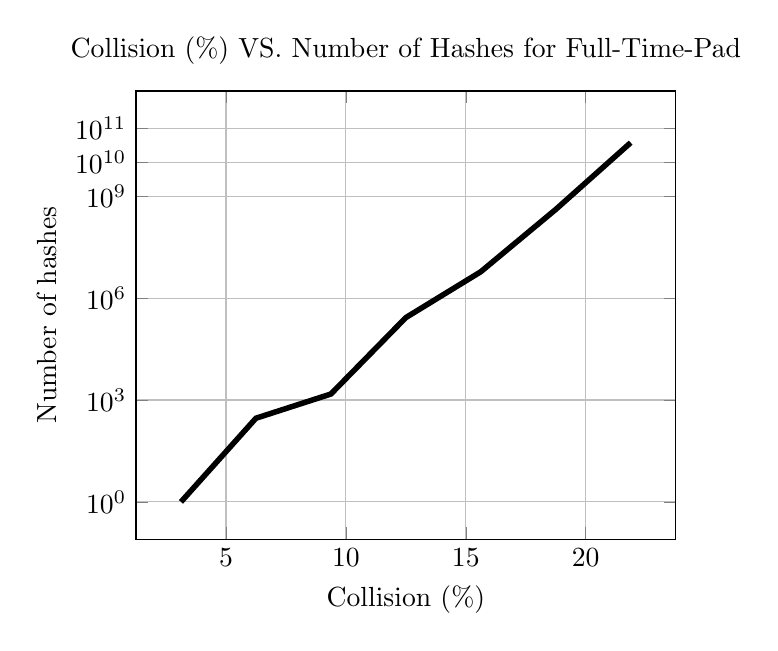
\begin{tikzpicture}
\begin{axis}[
    xlabel={Collision (\%)},
    ylabel={Number of hashes},
    title={Collision (\%) VS. Number of Hashes for Full-Time-Pad},
    ymode=log, 
    ymin=1,    
    ymax=1e11, 
    xtick distance=5,
    ytick distance=1,
    grid=major, 
    enlargelimits,
    legend style={at={(0.5,-0.15)}, anchor=north, legend columns=1},
    ytick={1, 1e3, 1e6, 1e9, 1e10, 1e11}, 
    yticklabel style={/pgf/number format/fixed},
]
    % Add the plot coordinates
    \addplot[line width=2pt] coordinates {
        (3.125, 1)
        (6.25, 291)
        (9.375, 1501)
        (12.5, 267184)
        (15.625, 5981439)
        (18.75, 408355721)
        (21.875, 37820493025)
    };
\end{axis}
\end{tikzpicture}%


\subsection{Differential Cryptoanalysis}

In \texttt{test/significant\_perm\_byte.cpp}, instead of comparing if values are equal, but rather approximately equal with accuracy of $\pm n$. This gave the same results are sha-256. And no specific bytes seemed to have followed a specific pattern. This means that there isn't a differential statistical pattern.

\begin{table}[h!]
\centering
\begin{tabular}{|c|c|c|}
\hline
\textbf{n} & \textbf{Full-Time-Pad (\%)} & \textbf{SHA-256 (\%)} \\
\hline
		0 & 0.3883 & 0.3923 \\
\hline
		5 & 4.2678 & 4.224 \\
\hline
		10 & 8.0342 & 8.0322 \\
\hline
		15 & 11.7421 & 11.7403 \\
\hline
		20 & 15.4626 & 15.4287 \\
\hline
		25 & 18.8071 & 18.8382 \\
\hline
\end{tabular}
\caption{Comparision Accuracy VS. Collision Rate}
\end{table}

Results of collision rates are approximately equal given lower accuracy ($\pm n$). This suggests that there isn't any cryptoanalysis pattern. These numbers are average of 255 tries. Each try also yields similar results which means that there isn't a differential cryptoanalysis exploit regarding accuracy of comparision.

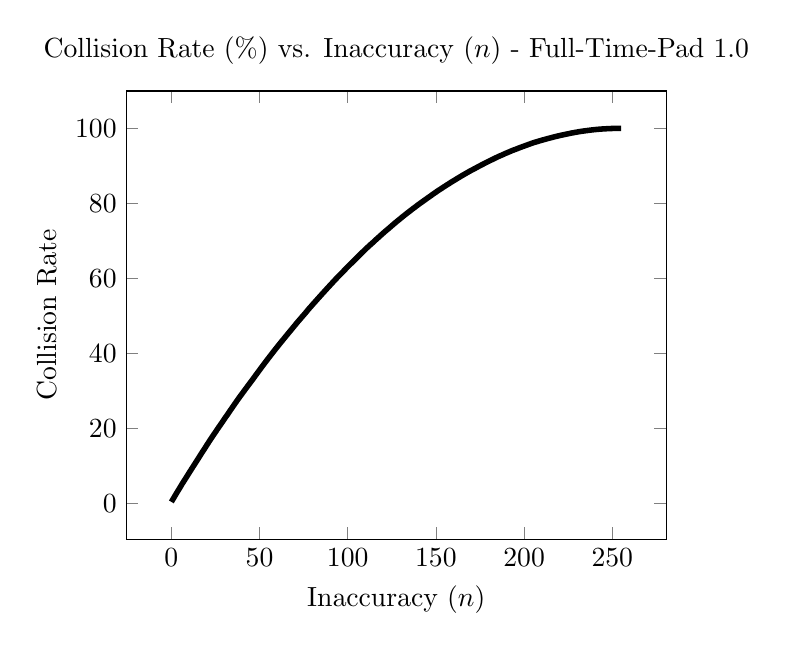
\begin{tikzpicture}
\begin{axis}[
	xlabel={Inaccuracy ($n$)},
	ylabel={Collision Rate},
	title={Collision Rate (\%) vs. Inaccuracy ($n$) - Full-Time-Pad 1.0}
]
    \addplot[line width=2pt] coordinates {
(0, 0.37186) (1, 1.1669) (2, 1.95964) (3, 2.74548) (4, 3.52865) (5, 4.29228) (6, 5.09536) (7, 5.83946) (8, 6.57169) (9, 7.31809) (10, 8.07751) (11, 8.80515) (12, 9.55767) (13, 10.2773) (14, 11.0244) (15, 11.7597) (16, 12.5019) (17, 13.2533) (18, 13.9729) (19, 14.6998) (20, 15.4481) (21, 16.1703) (22, 16.9091) (23, 17.6137) (24, 18.3088) (25, 18.9882) (26, 19.7074) (27, 20.3864) (28, 21.0662) (29, 21.7448) (30, 22.4472) (31, 23.1296) (32, 23.7818) (33, 24.4903) (34, 25.1769) (35, 25.8555) (36, 26.5391) (37, 27.2089) (38, 27.8799) (39, 28.534) (40, 29.1697) (41, 29.8028) (42, 30.4515) (43, 31.0796) (44, 31.7115) (45, 32.3369) (46, 32.963) (47, 33.6171) (48, 34.2605) (49, 34.9035) (50, 35.5342) (51, 36.1834) (52, 36.8087) (53, 37.4403) (54, 38.0507) (55, 38.6692) (56, 39.2827) (57, 39.8924) (58, 40.4971) (59, 41.093) (60, 41.6797) (61, 42.271) (62, 42.8627) (63, 43.4383) (64, 44.0058) (65, 44.586) (66, 45.1643) (67, 45.7307) (68, 46.2921) (69, 46.8716) (70, 47.4314) (71, 48.0124) (72, 48.5815) (73, 49.1042) (74, 49.6664) (75, 50.203) (76, 50.7418) (77, 51.3163) (78, 51.885) (79, 52.4085) (80, 52.9538) (81, 53.4739) (82, 53.9993) (83, 54.5282) (84, 55.0502) (85, 55.5748) (86, 56.0903) (87, 56.6142) (88, 57.1297) (89, 57.644) (90, 58.148) (91, 58.6596) (92, 59.1724) (93, 59.6729) (94, 60.167) (95, 60.6445) (96, 61.1198) (97, 61.6042) (98, 62.099) (99, 62.5862) (100, 63.0722) (101, 63.5355) (102, 63.9913) (103, 64.4631) (104, 64.9226) (105, 65.3918) (106, 65.8693) (107, 66.3343) (108, 66.8076) (109, 67.2603) (110, 67.703) (111, 68.1637) (112, 68.5784) (113, 69.0246) (114, 69.4286) (115, 69.8652) (116, 70.3052) (117, 70.7223) (118, 71.147) (119, 71.5782) (120, 71.9937) (121, 72.4127) (122, 72.8075) (123, 73.2012) (124, 73.6068) (125, 74.02) (126, 74.4259) (127, 74.825) 
(128, 75.2152) (129, 75.5936) (130, 75.9727) (131, 76.3714) (132, 76.7413) (133, 77.1205) (134, 77.4908) (135, 77.8431) (136, 78.2127) (137, 78.5735) (138, 78.9177) (139, 79.2819) (140, 79.6312) (141, 79.9805) (142, 80.3102) (143, 80.6472) (144, 80.9743) (145, 81.3243) (146, 81.6448) (147, 81.975) (148, 82.3254) (149, 82.6486) (150, 82.9722) (151, 83.3) (152, 83.6049) (153, 83.9101) (154, 84.2314) (155, 84.524) (156, 84.8353) (157, 85.1256) (158, 85.4331) (159, 85.728) (160, 86.0129) (161, 86.2944) (162, 86.5885) (163, 86.8723) (164, 87.153) (165, 87.4349) (166, 87.7003) (167, 87.9756) (168, 88.246) (169, 88.5172) (170, 88.7665) (171, 89.0131) (172, 89.2636) (173, 89.5133) (174, 89.776) (175, 90.0214) (176, 90.2616) (177, 90.5105) (178, 90.7502) (179, 90.993) (180, 91.2282) (181, 91.4614) (182, 91.6789) (183, 91.9141) (184, 92.1415) (185, 92.3698) (186, 92.585) (187, 92.7799) (188, 92.9875) (189, 93.2127) (190, 93.4141) (191, 93.6091) (192, 93.809) (193, 94.0135) (194, 94.1954) (195, 94.3712) (196, 94.5466) (197, 94.7396) (198, 94.9165) (199, 95.0869) (200, 95.2589) (201, 95.435) (202, 95.6028) (203, 95.7747) (204, 95.9432) (205, 96.0968) (206, 96.2626) (207, 96.3971) (208, 96.5303) (209, 96.6812) (210, 96.8195) (211, 96.952) (212, 97.068) (213, 97.2097) (214, 97.3357) (215, 97.4498) (216, 97.5793) (217, 97.6999) (218, 97.8159) (219, 97.9316) (220, 98.0438) (221, 98.1537) (222, 98.2541) (223, 98.3464) (224, 98.4494) (225, 98.5512) (226, 98.647) (227, 98.7458) (228, 98.83) (229, 98.9174) (230, 98.9993) (231, 99.0824) (232, 99.1613) (233, 99.2241) (234, 99.293) (235, 99.3574) (236, 99.4164) (237, 99.4795) (238, 99.5393) (239, 99.5948) (240, 99.6446) (241, 99.6952) (242, 99.735) (243, 99.7733) (244, 99.8097) (245, 99.8415) (246, 99.8637) (247, 99.8943) (248, 99.9169) (249, 99.941) (250, 99.954) (251, 99.9659) (252, 99.9812) (253, 99.9881) (254, 99.9939) (255, 100) 
	};
\end{axis}
\end{tikzpicture}

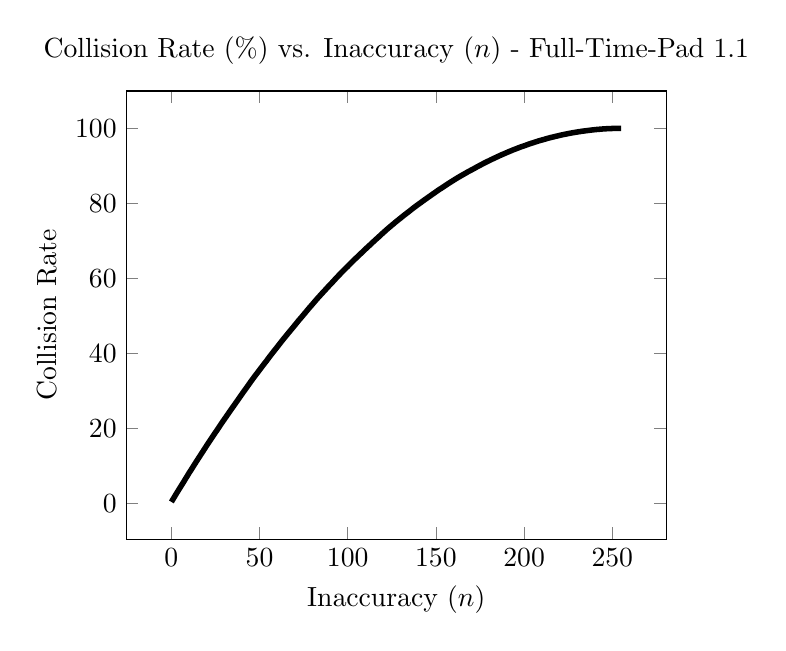
\begin{tikzpicture}
\begin{axis}[
	xlabel={Inaccuracy ($n$)},
	ylabel={Collision Rate},
	title={Collision Rate (\%) vs. Inaccuracy ($n$) - Full-Time-Pad 1.1}
]
    \addplot[line width=2pt] coordinates {
(0, 0.376072) (1, 1.15273) (2, 1.92632) (3, 2.7114) (4, 3.4869) (5, 4.23637) (6, 4.99157) (7, 5.74219) (8, 6.53378) (9, 7.27788) (10, 8.06411) (11, 8.78255) (12, 9.5278) (13, 10.2845) (14, 11.0198) (15, 11.754) (16, 12.4747) (17, 13.2135) (18, 13.9288) (19, 14.6638) (20, 15.3864) (21, 16.1137) (22, 16.7957) (23, 17.5207) (24, 18.2326) (25, 18.9131) (26, 19.604) (27, 20.3037) (28, 21.0248) (29, 21.7161) (30, 22.3836) (31, 23.0649) (32, 23.7446) (33, 24.421) (34, 25.1084) (35, 25.7663) (36, 26.4346) (37, 27.1067) (38, 27.7585) (39, 28.4498) (40, 29.1211) (41, 29.7882) (42, 30.4343) (43, 31.0934) (44, 31.7525) (45, 32.4292) (46, 33.0729) (47, 33.7155) (48, 34.3379) (49, 34.9514) (50, 35.5679) (51, 36.1926) (52, 36.8137) (53, 37.4234) (54, 38.0201) (55, 38.6669) (56, 39.29) (57, 39.9027) (58, 40.494) (59, 41.0869) (60, 41.6778) (61, 42.2855) (62, 42.8887) (63, 43.4926) (64, 44.0736) (65, 44.6392) (66, 45.2206) (67, 45.7966) (68, 46.3534) (69, 46.924) (70, 47.4931) (71, 48.0806) (72, 48.6669) (73, 49.2088) (74, 49.7587) (75, 50.3148) (76, 50.8747) (77, 51.4488) (78, 52.0209) (79, 52.5555) (80, 53.0852) (81, 53.637) (82, 54.1866) (83, 54.7243) (84, 55.2401) (85, 55.7709) (86, 56.2726) (87, 56.7804) (88, 57.3089) (89, 57.8079) (90, 58.3123) (91, 58.796) (92, 59.311) (93, 59.8296) (94, 60.3194) (95, 60.8287) (96, 61.3117) (97, 61.7923) (98, 62.2549) (99, 62.7248) (100, 63.1886) (101, 63.6742) (102, 64.167) (103, 64.6366) (104, 65.0823) (105, 65.522) (106, 65.9666) (107, 66.4235) (108, 66.867) (109, 67.3154) (110, 67.7658) (111, 68.207) (112, 68.637) (113, 69.0702) (114, 69.5213) (115, 69.9491) (116, 70.3968) (117, 70.792) (118, 71.2351) (119, 71.6808) (120, 72.1032) (121, 72.523) (122, 72.9523) (123, 73.3548) (124, 73.7546) (125, 74.1559) (126, 74.5408) (127, 74.9464) 
(128, 75.3213) (129, 75.702) (130, 76.0712) (131, 76.4557) (132, 76.834) (133, 77.1921) (134, 77.559) (135, 77.917) (136, 78.2908) (137, 78.6669) (138, 79.0165) (139, 79.3719) (140, 79.7124) (141, 80.0471) (142, 80.3964) (143, 80.7364) (144, 81.0685) (145, 81.4043) (146, 81.7383) (147, 82.0653) (148, 82.402) (149, 82.7152) (150, 83.0549) (151, 83.3873) (152, 83.7021) (153, 84.0047) (154, 84.3168) (155, 84.6289) (156, 84.938) (157, 85.2627) (158, 85.5461) (159, 85.8452) (160, 86.1455) (161, 86.4338) (162, 86.721) (163, 86.9975) (164, 87.2798) (165, 87.5517) (166, 87.8106) (167, 88.0821) (168, 88.3636) (169, 88.6091) (170, 88.858) (171, 89.115) (172, 89.3559) (173, 89.6366) (174, 89.8866) (175, 90.1329) (176, 90.3833) (177, 90.6411) (178, 90.8663) (179, 91.1121) (180, 91.3289) (181, 91.5702) (182, 91.7923) (183, 92.0148) (184, 92.2323) (185, 92.4521) (186, 92.6685) (187, 92.8925) (188, 93.0821) (189, 93.2931) (190, 93.4907) (191, 93.6994) (192, 93.8902) (193, 94.0889) (194, 94.2831) (195, 94.4577) (196, 94.6431) (197, 94.8273) (198, 95.0027) (199, 95.1693) (200, 95.329) (201, 95.4921) (202, 95.6698) (203, 95.8375) (204, 95.9938) (205, 96.1363) (206, 96.2994) (207, 96.4503) (208, 96.6035) (209, 96.7352) (210, 96.8708) (211, 96.9964) (212, 97.1339) (213, 97.2744) (214, 97.4054) (215, 97.5283) (216, 97.6386) (217, 97.7462) (218, 97.8692) (219, 97.9776) (220, 98.0913) (221, 98.2024) (222, 98.2973) (223, 98.3984) (224, 98.4926) (225, 98.5884) (226, 98.6814) (227, 98.7661) (228, 98.8473) (229, 98.9288) (230, 99.0081) (231, 99.0813) (232, 99.1517) (233, 99.2256) (234, 99.2865) (235, 99.3482) (236, 99.4083) (237, 99.465) (238, 99.527) (239, 99.5822) (240, 99.6312) (241, 99.681) (242, 99.7223) (243, 99.7595) (244, 99.8032) (245, 99.8365) (246, 99.8644) (247, 99.8932) (248, 99.9157) (249, 99.9334) (250, 99.9537) (251, 99.9682) (252, 99.9828) (253, 99.99) (254, 99.9962) (255, 100)
	};
\end{axis}
\end{tikzpicture}

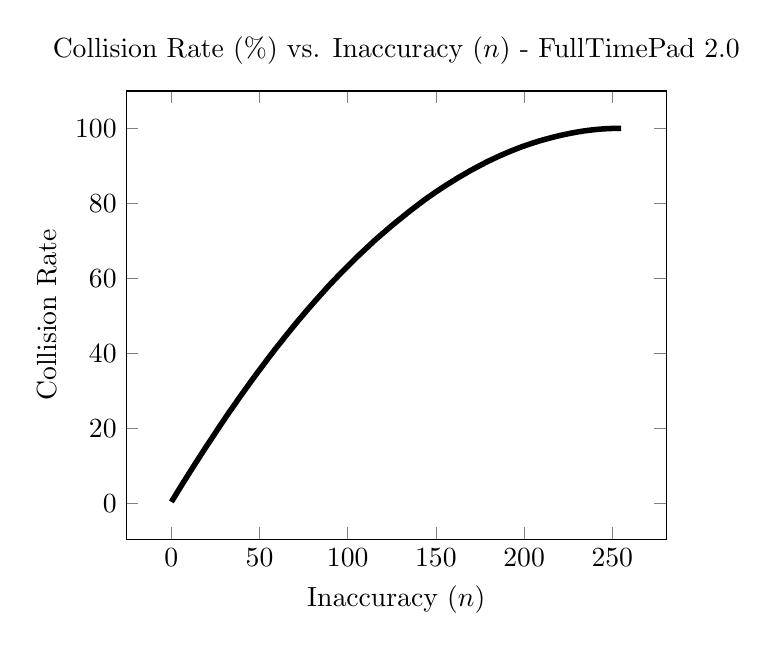
\begin{tikzpicture}
\begin{axis}[
	xlabel={Inaccuracy ($n$)},
	ylabel={Collision Rate},
	title={Collision Rate (\%) vs. Inaccuracy ($n$) - FullTimePad 2.0}
]
    \addplot[line width=2pt] coordinates {
%(0, 0.401348) (1, 1.19217) (2, 1.9918) (3, 2.7608) (4, 3.5252) (5, 4.30109) (6, 5.0337) (7, 5.78508) (8, 6.53952) (9, 7.3449) (10, 8.09628) (11, 8.82008) (12, 9.56725) (13, 10.3244) (14, 11.0938) (15, 11.8172) (16, 12.5452) (17, 13.2701) (18, 14.0058) (19, 14.7281) (20, 15.4584) (21, 16.1837) (22, 16.8957) (23, 17.6) (24, 18.3176) (25, 19.0158) (26, 19.707) (27, 20.4213) (28, 21.1278) (29, 21.8187) (30, 22.4824) (31, 23.1675) (32, 23.8392) (33, 24.5328) (34, 25.2336) (35, 25.8946) (36, 26.5954) (37, 27.2522) (38, 27.9285) (39, 28.5991) (40, 29.2682) (41, 29.9269) (42, 30.5683) (43, 31.188) (44, 31.8114) (45, 32.4487) (46, 33.1043) (47, 33.7504) (48, 34.3915) (49, 35.0341) (50, 35.6541) (51, 36.2948) (52, 36.9175) (53, 37.5421) (54, 38.1621) (55, 38.7657) (56, 39.3673) (57, 39.9602) (58, 40.5626) (59, 41.1581) (60, 41.7758) (61, 42.3595) (62, 42.9469) (63, 43.5355) (64, 44.1023) (65, 44.7005) (66, 45.2788) (67, 45.8567) (68, 46.3917) (69, 46.9692) (70, 47.5375) (71, 48.1204) (72, 48.6903) (73, 49.2593) (74, 49.792) (75, 50.3297) (76, 50.8667) (77, 51.3821) (78, 51.919) (79, 52.4885) (80, 53.0101) (81, 53.5382) (82, 54.0675) (83, 54.5872) (84, 55.0892) (85, 55.6059) (86, 56.1416) (87, 56.6847) (88, 57.1814) (89, 57.6861) (90, 58.2073) (91, 58.7155) (92, 59.2019) (93, 59.7112) (94, 60.2305) (95, 60.7131) (96, 61.227) (97, 61.726) (98, 62.1955) (99, 62.6727) (100, 63.1564) (101, 63.6393) (102, 64.1284) (103, 64.5906) (104, 65.0352) (105, 65.4921) (106, 65.9337) (107, 66.4051) (108, 66.8459) (109, 67.2871) (110, 67.7294) (111, 68.1801) (112, 68.6275) (113, 69.0453) (114, 69.4903) (115, 69.9062) (116, 70.337) (117, 70.7878) (118, 71.1991) (119, 71.6291) (120, 72.0485) (121, 72.4468) (122, 72.8715) (123, 73.2824) (124, 73.6684) (125, 74.056) (126, 74.4723) (127, 74.8587) 
%(128, 75.2313) (129, 75.6304) (130, 76.0279) (131, 76.4047) (132, 76.7965) (133, 77.1557) (134, 77.5352) (135, 77.8814) (136, 78.2525) (137, 78.6163) (138, 78.9721) (139, 79.3222) (140, 79.6806) (141, 80.0195) (142, 80.3627) (143, 80.7211) (144, 81.0838) (145, 81.4288) (146, 81.7666) (147, 82.0607) (148, 82.3916) (149, 82.7014) (150, 83.0205) (151, 83.3375) (152, 83.6619) (153, 83.9748) (154, 84.277) (155, 84.5929) (156, 84.9077) (157, 85.1984) (158, 85.4971) (159, 85.7939) (160, 86.0895) (161, 86.3848) (162, 86.6785) (163, 86.9573) (164, 87.2415) (165, 87.5134) (166, 87.7926) (167, 88.0519) (168, 88.3188) (169, 88.5784) (170, 88.8281) (171, 89.0977) (172, 89.349) (173, 89.622) (174, 89.8736) (175, 90.1153) (176, 90.3811) (177, 90.6196) (178, 90.8398) (179, 91.0765) (180, 91.3182) (181, 91.5594) (182, 91.798) (183, 92.0201) (184, 92.2327) (185, 92.4563) (186, 92.6739) (187, 92.8918) (188, 93.0944) (189, 93.2927) (190, 93.5061) (191, 93.7121) (192, 93.9193) (193, 94.1081) (194, 94.3084) (195, 94.4964) (196, 94.6798) (197, 94.861) (198, 95.0471) (199, 95.2145) (200, 95.3864) (201, 95.5507) (202, 95.715) (203, 95.8678) (204, 96.0141) (205, 96.1788) (206, 96.3201) (207, 96.4557) (208, 96.6065) (209, 96.731) (210, 96.8781) (211, 97.0133) (212, 97.1481) (213, 97.2825) (214, 97.4066) (215, 97.5222) (216, 97.6444) (217, 97.7673) (218, 97.8841) (219, 97.9979) (220, 98.1059) (221, 98.2104) (222, 98.3115) (223, 98.4103) (224, 98.5214) (225, 98.6232) (226, 98.7063) (227, 98.7937) (228, 98.8771) (229, 98.9698) (230, 99.0537) (231, 99.1238) (232, 99.1919) (233, 99.2613) (234, 99.3241) (235, 99.3853) (236, 99.4481) (237, 99.5006) (238, 99.5512) (239, 99.5998) (240, 99.6465) (241, 99.6955) (242, 99.7381) (243, 99.7775) (244, 99.8066) (245, 99.8418) (246, 99.8671) (247, 99.8932) (248, 99.9142) (249, 99.9345) (250, 99.954) (251, 99.9686) (252, 99.9809) (253, 99.9916) (254, 99.9966) (255, 100)
(0, 0.384881) (1, 1.15119) (2, 1.89836) (3, 2.68765) (4, 3.45014) (5, 4.21109) (6, 4.98009) (7, 5.72457) (8, 6.4591) (9, 7.21201) (10, 7.98483) (11, 8.70864) (12, 9.44317) (13, 10.1827) (14, 10.9291) (15, 11.6498) (16, 12.3729) (17, 13.1085) (18, 13.8454) (19, 14.5745) (20, 15.3006) (21, 15.9992) (22, 16.69) (23, 17.4043) (24, 18.125) (25, 18.8304) (26, 19.545) (27, 20.2665) (28, 20.9651) (29, 21.659) (30, 22.3564) (31, 23.0771) (32, 23.7722) (33, 24.4405) (34, 25.0965) (35, 25.7809) (36, 26.4396) (37, 27.1251) (38, 27.8136) (39, 28.4697) (40, 29.128) (41, 29.776) (42, 30.4454) (43, 31.0834) (44, 31.7494) (45, 32.4069) (46, 33.0373) (47, 33.6807) (48, 34.326) (49, 34.9824) (50, 35.5909) (51, 36.2201) (52, 36.8451) (53, 37.4671) (54, 38.1047) (55, 38.7477) (56, 39.3608) (57, 39.9671) (58, 40.5699) (59, 41.1857) (60, 41.7793) (61, 42.3671) (62, 42.9419) (63, 43.5386) (64, 44.1513) (65, 44.7373) (66, 45.3048) (67, 45.8988) (68, 46.4725) (69, 47.0496) (70, 47.6191) (71, 48.1916) (72, 48.7787) (73, 49.3137) (74, 49.8709) (75, 50.427) (76, 50.9666) (77, 51.5368) (78, 52.0764) (79, 52.6007) (80, 53.1407) (81, 53.6845) (82, 54.2149) (83, 54.7522) (84, 55.2597) (85, 55.7904) (86, 56.3009) (87, 56.8313) (88, 57.3602) (89, 57.8734) (90, 58.3996) (91, 58.8752) (92, 59.3696) (93, 59.8621) (94, 60.3512) (95, 60.8487) (96, 61.335) (97, 61.7953) (98, 62.2488) (99, 62.7263) (100, 63.2119) (101, 63.7033) (102, 64.1602) (103, 64.635) (104, 65.0934) (105, 65.5653) (106, 66.0118) (107, 66.4714) (108, 66.9037) (109, 67.3415) (110, 67.7746) (111, 68.2261) (112, 68.6719) (113, 69.1104) (114, 69.5424) (115, 69.9759) (116, 70.4056) (117, 70.8119) (118, 71.2152) (119, 71.6307) (120, 72.0397) (121, 72.4299) (122, 72.8454) (123, 73.2445) (124, 73.6562) (125, 74.043) (126, 74.4462) (127, 74.8242)
(128, 75.2034) (129, 75.5848) (130, 75.9532) (131, 76.3312) (132, 76.7149) (133, 77.0941) (134, 77.4893) (135, 77.8542) (136, 78.2303) (137, 78.5735) (138, 78.9365) (139, 79.2904) (140, 79.6618) (141, 80.0069) (142, 80.3638) (143, 80.7181) (144, 81.0696) (145, 81.4043) (146, 81.7398) (147, 82.0558) (148, 82.3932) (149, 82.7229) (150, 83.0446) (151, 83.3548) (152, 83.6638) (153, 83.9798) (154, 84.2819) (155, 84.5841) (156, 84.8863) (157, 85.1949) (158, 85.4753) (159, 85.7663) (160, 86.0673) (161, 86.3519) (162, 86.6559) (163, 86.9363) (164, 87.2105) (165, 87.4793) (166, 87.7363) (167, 88.0109) (168, 88.3004) (169, 88.5819) (170, 88.8369) (171, 89.0832) (172, 89.3283) (173, 89.5906) (174, 89.8319) (175, 90.0896) (176, 90.3282) (177, 90.5729) (178, 90.8318) (179, 91.0646) (180, 91.3036) (181, 91.5066) (182, 91.7448) (183, 91.9619) (184, 92.1871) (185, 92.4096) (186, 92.6203) (187, 92.8351) (188, 93.0369) (189, 93.2349) (190, 93.4341) (191, 93.6386) (192, 93.8392) (193, 94.0234) (194, 94.2142) (195, 94.398) (196, 94.5925) (197, 94.7729) (198, 94.9502) (199, 95.1153) (200, 95.2849) (201, 95.453) (202, 95.6166) (203, 95.7629) (204, 95.9237) (205, 96.0849) (206, 96.2316) (207, 96.3848) (208, 96.5269) (209, 96.6785) (210, 96.8133) (211, 96.9436) (212, 97.0734) (213, 97.2013) (214, 97.3235) (215, 97.4468) (216, 97.5789) (217, 97.6945) (218, 97.8125) (219, 97.9236) (220, 98.04) (221, 98.1403) (222, 98.2506) (223, 98.3525) (224, 98.4528) (225, 98.5616) (226, 98.6531) (227, 98.7358) (228, 98.8212) (229, 98.9089) (230, 98.9939) (231, 99.0778) (232, 99.1464) (233, 99.2341) (234, 99.2961) (235, 99.3658) (236, 99.4171) (237, 99.4838) (238, 99.5339) (239, 99.5937) (240, 99.6408) (241, 99.6837) (242, 99.7258) (243, 99.7706) (244, 99.8116) (245, 99.846) (246, 99.874) (247, 99.902) (248, 99.9269) (249, 99.9445) (250, 99.9606) (251, 99.972) (252, 99.9812) (253, 99.992) (254, 99.9969) (255, 100)


	};
\end{axis}
\end{tikzpicture}



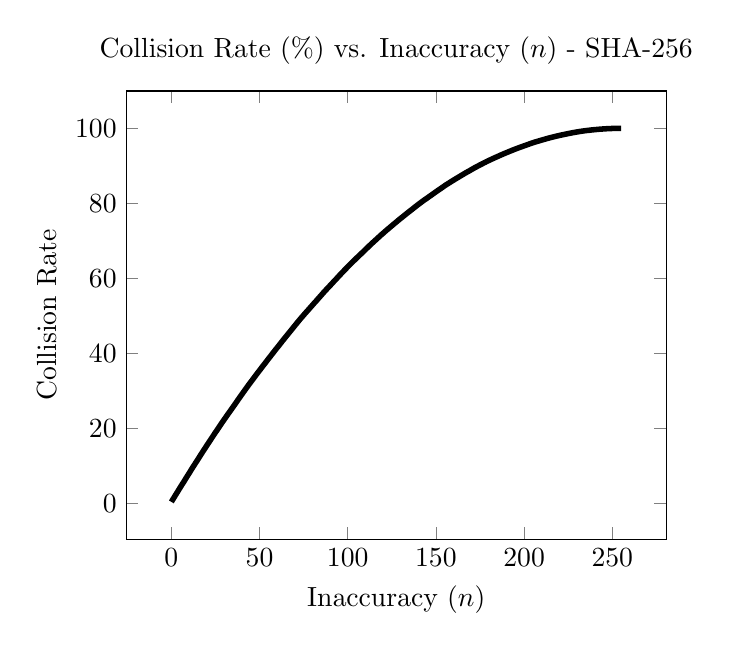
\begin{tikzpicture}
\begin{axis}[
	xlabel={Inaccuracy ($n$)},
	ylabel={Collision Rate},
	title={Collision Rate (\%) vs. Inaccuracy ($n$) - SHA-256}
]
    \addplot[line width=2pt] coordinates {( 0 ,  0.3703) ( 1 ,  1.1527) ( 2 ,  1.9259) ( 3 ,  2.6823) ( 4 ,  3.4501) ( 5 ,  4.2168) ( 6 ,  4.9732) ( 7 ,  5.6932) ( 8 ,  6.471) ( 9 ,  7.2315) ( 10 ,  7.9592) ( 11 ,  8.7385) ( 12 ,  9.4968) ( 13 ,  10.2225) ( 14 ,  10.9536) ( 15 ,  11.6759) ( 16 ,  12.4303) ( 17 ,  13.1775) ( 18 ,  13.8997) ( 19 ,  14.6109) ( 20 ,  15.3508) ( 21 ,  16.0432) ( 22 ,  16.777) ( 23 ,  17.4874) ( 24 ,  18.1928) ( 25 ,  18.9074) ( 26 ,  19.5879) ( 27 ,  20.2899) ( 28 ,  21.0114) ( 29 ,  21.6973) ( 30 ,  22.3663) ( 31 ,  23.0515) ( 32 ,  23.7167) ( 33 ,  24.383) ( 34 ,  25.0375) ( 35 ,  25.7104) ( 36 ,  26.3657) ( 37 ,  27.0573) ( 38 ,  27.739) ( 39 ,  28.4027) ( 40 ,  29.0717) ( 41 ,  29.7266) ( 42 ,  30.3937) ( 43 ,  31.0424) ( 44 ,  31.6916) ( 45 ,  32.315) ( 46 ,  32.9362) ( 47 ,  33.5731) ( 48 ,  34.218) ( 49 ,  34.8242) ( 50 ,  35.4373) ( 51 ,  36.0666) ( 52 ,  36.6839) ( 53 ,  37.2679) ( 54 ,  37.8868) ( 55 ,  38.5087) ( 56 ,  39.0973) ( 57 ,  39.7243) ( 58 ,  40.3075) ( 59 ,  40.9268) ( 60 ,  41.5097) ( 61 ,  42.0929) ( 62 ,  42.6972) ( 63 ,  43.3088) ( 64 ,  43.8821) ( 65 ,  44.4684) ( 66 ,  45.0494) ( 67 ,  45.63) ( 68 ,  46.1991) ( 69 ,  46.79) ( 70 ,  47.3752) ( 71 ,  47.9569) ( 72 ,  48.5306) ( 73 ,  49.0977) ( 74 ,  49.6484) ( 75 ,  50.1792) ( 76 ,  50.7338) ( 77 ,  51.2481) ( 78 ,  51.7839) ( 79 ,  52.325) ( 80 ,  52.8466) ( 81 ,  53.385) ( 82 ,  53.8963) ( 83 ,  54.4374) ( 84 ,  54.974) ( 85 ,  55.4952) ( 86 ,  56.0459) ( 87 ,  56.5656) ( 88 ,  57.0699) ( 89 ,  57.5735) ( 90 ,  58.0695) ( 91 ,  58.5719) ( 92 ,  59.0901) ( 93 ,  59.5807) ( 94 ,  60.0908) ( 95 ,  60.6101) ( 96 ,  61.1003) ( 97 ,  61.6) ( 98 ,  62.0921) ( 99 ,  62.572) ( 100 ,  63.0691) ( 101 ,  63.5401) ( 102 ,  64.0008) ( 103 ,  64.4807) ( 104 ,  64.9249) ( 105 ,  65.396) ( 106 ,  65.841) ( 107 ,  66.2829) ( 108 ,  66.7325) ( 109 ,  67.1852) ( 110 ,  67.6559) ( 111 ,  68.0924) ( 112 ,  68.5597) ( 113 ,  68.9959) ( 114 ,  69.4405) ( 115 ,  69.8644) ( 116 ,  70.2953) ( 117 ,  70.7265) ( 118 ,  71.1558) ( 119 ,  71.5874) ( 120 ,  71.9857) ( 121 ,  72.4131) ( 122 ,  72.8236) ( 123 ,  73.2081) ( 124 ,  73.6144) ( 125 ,  74.0127) ( 126 ,  74.4076) ( 127 ,  74.7982) ( 128 ,  75.1888) ( 129 ,  75.589) ( 130 ,  75.9746) ( 131 ,  76.335) ( 132 ,  76.7214) ( 133 ,  77.1052) ( 134 ,  77.4774) ( 135 ,  77.8435) ( 136 ,  78.2093) ( 137 ,  78.5777) ( 138 ,  78.958) ( 139 ,  79.321) ( 140 ,  79.6871) ( 141 ,  80.0429) ( 142 ,  80.396) ( 143 ,  80.7395) ( 144 ,  81.0612) ( 145 ,  81.3825) ( 146 ,  81.7291) ( 147 ,  82.0427) ( 148 ,  82.384) ( 149 ,  82.7259) ( 150 ,  83.0538) ( 151 ,  83.3847) ( 152 ,  83.701) ( 153 ,  84.0246) ( 154 ,  84.3604) ( 155 ,  84.6806) ( 156 ,  84.9958) ( 157 ,  85.2953) ( 158 ,  85.5875) ( 159 ,  85.8912) ( 160 ,  86.1765) ( 161 ,  86.4656) ( 162 ,  86.744) ( 163 ,  87.0351) ( 164 ,  87.3135) ( 165 ,  87.5957) ( 166 ,  87.8761) ( 167 ,  88.1541) ( 168 ,  88.4099) ( 169 ,  88.6688) ( 170 ,  88.9491) ( 171 ,  89.2172) ( 172 ,  89.4857) ( 173 ,  89.7319) ( 174 ,  89.9805) ( 175 ,  90.2344) ( 176 ,  90.4714) ( 177 ,  90.7192) ( 178 ,  90.9436) ( 179 ,  91.188) ( 180 ,  91.4101) ( 181 ,  91.6311) ( 182 ,  91.8539) ( 183 ,  92.0722) ( 184 ,  92.2763) ( 185 ,  92.4862) ( 186 ,  92.6968) ( 187 ,  92.9094) ( 188 ,  93.1147) ( 189 ,  93.3142) ( 190 ,  93.5045) ( 191 ,  93.6983) ( 192 ,  93.8909) ( 193 ,  94.0908) ( 194 ,  94.2747) ( 195 ,  94.4589) ( 196 ,  94.635) ( 197 ,  94.8108) ( 198 ,  94.9851) ( 199 ,  95.1478) ( 200 ,  95.324) ( 201 ,  95.4822) ( 202 ,  95.6618) ( 203 ,  95.828) ( 204 ,  95.9969) ( 205 ,  96.1443) ( 206 ,  96.2998) ( 207 ,  96.4522) ( 208 ,  96.587) ( 209 ,  96.7218) ( 210 ,  96.8635) ( 211 ,  96.9945) ( 212 ,  97.1312) ( 213 ,  97.2652) ( 214 ,  97.392) ( 215 ,  97.5234) ( 216 ,  97.6398) ( 217 ,  97.7593) ( 218 ,  97.8726) ( 219 ,  97.9783) ( 220 ,  98.0947) ( 221 ,  98.1909) ( 222 ,  98.292) ( 223 ,  98.3927) ( 224 ,  98.4953) ( 225 ,  98.5903) ( 226 ,  98.6834) ( 227 ,  98.7737) ( 228 ,  98.8607) ( 229 ,  98.9445) ( 230 ,  99.0296) ( 231 ,  99.1065) ( 232 ,  99.1793) ( 233 ,  99.2544) ( 234 ,  99.3168) ( 235 ,  99.383) ( 236 ,  99.4363) ( 237 ,  99.4861) ( 238 ,  99.5447) ( 239 ,  99.5906) ( 240 ,  99.6381) ( 241 ,  99.6841) ( 242 ,  99.7227) ( 243 ,  99.7683) ( 244 ,  99.8024) ( 245 ,  99.8346) ( 246 ,  99.8637) ( 247 ,  99.8932) ( 248 ,  99.9146) ( 249 ,  99.938) ( 250 ,  99.9548) ( 251 ,  99.9663) ( 252 ,  99.9793) ( 253 ,  99.9889) ( 254 ,  99.9954) ( 255 ,  100.0)};
\end{axis}
\end{tikzpicture}


This graph demonstrates how lower accuracy of comparison results in higher collision rate (For both SHA-256 and Full-Time-Pad). The points for this graph is evaluated by running \texttt{test/significant\_perm\_byte -d}. The consistent non-volatile increase in the numbers are a good thing.
\\
\subsection{Reverse Engineering the Transformation}

this is demonstrated in the \texttt{test/reverse.cpp} code. The reversed key and key are very different.

\subsection{Collision-Resistance}

Collision resistance has been proven in the birthday problem section and the collision attack section. The collision resistance is on average about as low as the numbers in sha256. and don't have any particular patterns as proven in \texttt{test/significant\_perm\_byte.cpp}. This test file shows the collision rate as any byte of the 32-byte key is modified by 1-bit.
\\\\
$\texttt{collision\_rate} = \frac{\texttt{\#collisions}}{\texttt{32}}$\\
 \\ where \texttt{\#collisions} is the number of bytes where $\texttt{previous key}_i$ and $\texttt{modified key}_i$ are equal

\subsubsection{Different Permutation Matrices}

Tried permutation matrices that followed logic or randomness. But they didn't offer the proper diffusion and collision resistance required to make a secure algrorithm. The permutation matrix needs to be perfect so that the chances of collision (tested in \texttt{test/significant\_perm\_byte.cpp}) for every byte of the key should be around the same.\\
Using Bent functions to generate a non-uniform permutation matrix is also possible.

In terms of efficiency, the permutation matrix should be a uniform permutation matrix. The current matrix is non-uniform, which might provide better diffusion (more random), it also creates the issue of efficiency. So in terms of computation speed, reducing the number of times the memory is accessed is required. To achieve this, I will implement an updated version with uniform matrix and perform benchmark tests, based on results of both avalanche effect and cryptoanalysis testing, I will keep/undo the tests.

\subsubsection{Number of Rounds}

Number of rounds is determined by the number of rows in the permutation matrix. as using a permutation twice will cancel out.

\subsubsection{Constant - $F_p$ - Prime Galois Field Size}

every addition operation is done in a prime galois field as every $k_i \in \mathbb{F_p}$ where $k_i$ is the i'th index of the 32-bit segmented key $p = \texttt{0xfffffffb}$. p is the largest unsigned 32-bit prime number. It was evaluated using Fermat's Little Theorem:\\
\\
\begin{algorithm}[H] % H is to make the algorithm stay HERE
\caption{Find the largest 32-bit prime number pseudo-code}
\begin{algorithmic}[1]  % The [1] enables line numbering
\State \textbf{Output:} Biggest unsigned 32-bit prime number ($p$)
\State \textbf{Begin}
\State $p = 0$
\For{$i = \texttt{0xffffffff}$ to $0$}
	\If {$2^{i-1} \mod i = 1$}
		\State $p = i$
		\State break
	\EndIf
\EndFor
\State \textbf{Return} $p$
\end{algorithmic}
\end{algorithm}

\subsubsection{Constant - $r$ - Dynamic Rotation Constant} \label{rotation_constant}

Cicadas only surface once every 17 years. Assuming that their predetor only surfaces once every 2 years, they will only meet each other once every 34 years. Since 17 is a prime number, they will barely ever meet. However, if they surfaced once every 18 years, while their predetor once every 2 years. Then every 18 years they would meet. This would also make it easier for the predetor to synchronize their emergence timing.\\
let x be the time interval for when the cicadas surface \\
let y be the time interval for when the predetors surface \\
We can conclude:\\
$GCD(x,y) = 1$, then they meet up every $x \times y$ years. \\
Whereas if $GCD(x,y) \neq 1$, then they meet up every $x$ years (assuming $x > y$). \\
\\
Bitwise rotation operation should also be done with either a prime number or a number where $GCD(x,y) = 1$ to maximize the collision resistance.\\

If not, then for example: \\
let $w$ be 32-bit number\\
let $q = 8$ be rotation count\\
rotation can be represented by: $w = w \lll q$\\
If this rotation was repeated for 4 iterations, then the rotations would cancel out and rotated $w$ ($w'$) and $w$ would be equal. Make sure that $GCD(q, 32) = 1$. \\

If there's only one rotation number, the likelihood of finding a pattern increases. Imagine a card dealer shuffling cards with two stacks, ensuring that one card from each stack is placed on top of the other in a consistent pattern. In this case, you could easily "unshuffle" the cards by simply separating them into two stacks, putting one card on one side and one card on the other. Using a single rotation like this is too simple, but if the cards were shuffled using a more complex method, the process becomes harder to reverse. Even though each method is reversible on its own, combining them makes it significantly more difficult to undo. The use of bitwise rotations on 32-bit segments combined with byte-level permutations creates excellent diffusion. The only potential improvement would be to ensure that all bytes are interlinked solely through the bitwise rotations and permutations, rather than relying on the sum, as seen in the current transformation algorithm.

Rotation numbers that are selected are represented by r:

\[
r = 
\begin{pmatrix}
		23 & 5 & 17 & 31 & 13
\end{pmatrix}
\]

There are 5 numbers for r, this is because $16 \mod 5 \neq 0$, after 16 iterations in the transformation algorithm, all values of k aren't rotated the same number of times.

If you were to rotate 32-bit unsigned integer (x)
\[
\sum_{i=0}^4 r_i = 89
\]
\\
number of times, the net rotation would be 89 (a prime number). $x \ggg 89$ would produce a net rotation of $x \ggg 25$, since $89 \mod 32=25$. Knowing that $GCD(25, 32) = 1$, the minimum number of times where the expression $x \ggg 89$ is repeated till rotated $x$ equals $x$ is $89 \times 32 = 2848$. This means that only after $2848$ iterations would rotated x equal x. Whereas if there was a singular number for $r$, the number of rotations for rotated $x$ to equal $x$ would be $r \times 32$ (e.g. $r=23, 23 \times 32 = 736$). \\

$\therefore$ there needs to be multiple numbers for r.
\\
It is designed so that $|r_i - r_{i-1}|$ results in a different magnitude each time so that the net rotation is a bigger number (more rotation means better diffusion/confusion).
\\
For the deravation, the numbers started with prime numbers, all prime numbers from 0-32, but most were eliminated due to similiar values for  $|r_i - r_{i-1}|$ results (e.g. $23-5=18$, $|5-17|=12$ aren't too close). A good net rotation would be prime and without similiarities to net rotations. In the transformation algorithm, There are bitwise right rotate ($\ggg$) and bitwise left rotate ($\lll$), this is done to properly mix the results.

\section{Hashing}

The 'hashing' algorithm is used for manipulating the key each time with proper confusion and avalanche effect. The main reason why the key can be reused is due to the algorithm's strong avalanche effect as well as the lack of statistical patterns with collision rates as proven in the unit tests, \texttt{test/significant\_perm\_byte.cpp} which shows if some bytes have more or less collision reasistance.
\\
To maximize the effects of confusion using the current logic, 4 out of 8 values k (32-bit segmented key) should be modified per iteration (half of key). So each byte of the key is transformed a total of 8 times ($\frac{16 \texttt{iterations}}{8 \div 4}$). since $16 \mod 4 = 0$, all bytes are transformed the same number of times which would also tarnish the possibility of a statistical exploit that could target less transformed bytes of the key.
\\
Half of the key should be modified per iteration because classical cryptographic algorithms (non-quantum) rely on computational complexity for their security. So more transformation the better. But the most minimum work to get a secure transformed key is enough, \\
therefore it's the goal. this was determined experimentally; testing collision resistance of each byte upon modifying the transformation algorithm. \\
\\

I would represent the transformation algorithm with a game of cards. Imagine that 8 cards are randomly picked in a pile of $2^{256}$ cards, each card is cut up into 4 equal pieces, the cut up pieces are shuffled using a permutation algorithm while also replaced with other cut up values from the pile of cards and simultaniously, some pieces are cut up to 2 pieces with magnitude of a prime number (e.g. 5mm, other pieces being 32-5mm if card is 32mm). If this process repeated for 16 iterations, could you recover the original cards? Probably not.

\subsection{Dynamic Matrix Permutation}

Considering the use of \texttt{reinterpret\_cast} for representing the bytearray (key) as 32-bit segments (for confusion operations), the endiannes of the computer will affect the matrix. the matrix given in this documentation is the big endian version as the algorithm is designed to be big-endian. The little endian version requires a new permutation matrix where the byte order every 32-bits is reversed. This is in the C++ implementation of \texttt{Full-Time-Pad} and the python Deravation program mentioned below.
\\
This generates a non-uniform permutation matrix. Which is a "key" concept in uniform randomization of the transposition of bytes.

\subsubsection{Deravation}

\begin{algorithm}[H] % H is to make the algorithm stay HERE
\caption{Dynamic Permutation Matrix Deravation Pseudo-code}
\begin{algorithmic}[1]  % The [1] enables line numbering
\State \textbf{Input:} an array of incrementing numbers (0-31) $A$ 
\State \textbf{Output:} Most Efficient Permutation Matrix $V$ ($16 \times 32$)
\State \textbf{Begin}
\State $P \gets \texttt{copy of A}$
\For{$k = 0$ to $4$}
	\For{$i = 0$ to $8$}
		\State $P_i      \gets A_{i \times 4}$
		\State $P_{i+8}  \gets A_{i \times 4 + 1}$
		\State $P_{i+16} \gets A_{i \times 4 + 2}$
		\State $P_{i+24} \gets A_{i \times 4 + 3}$
	\EndFor
	\State $A \gets \texttt{copy of P}$
	\State $V.append(P)$
	\State $C \gets \texttt{copy of P}$
	\For{$m = 0$ to $3$}
		\For{$i = 0$ to $8$}
			\For{$n = 0$ to $4$}
			\State $P_{i \times 4 + n} \gets C_{(1+n+m) \mod{4} \texttt{    } + \texttt{    } i \times 4}$
			\EndFor
		\EndFor
		\State $V.append(P)$
	\EndFor
	\State $A \gets \texttt{copy of P}$
\EndFor
\State \textbf{Return} $V$
\end{algorithmic}
\end{algorithm}

Python code is in the test/perm.py
 
\subsubsection{Dynamic Permutation Matrix Values} % include Discovery

\renewcommand{\arraystretch}{1} % Decrease vertical space between rows 

\small
\[
\begin{Bmatrix}
\phantom{0}0 & \phantom{0}4 & \phantom{0}8 & 12 & 16 & 20 & 24 & 28 & \phantom{0}1 & \phantom{0}5 & 9 & 13 & 17 & 21 & 25 & 29 & \phantom{0}2 & \phantom{0}6 & 10 & 14 & 18 & 22 & 26 & 30 & \phantom{0}3 & \phantom{0}7 & 11 & 15 & 19 & 23 & 27 & 31 \\
\phantom{0}4 & \phantom{0}8 & 12 & \phantom{0}0 & 20 & 24 & 28 & 16 & \phantom{0}5 & 9 & 13 & \phantom{0}1 & 21 & 25 & 29 & 17 & \phantom{0}6 & 10 & 14 & \phantom{0}2 & 22 & 26 & 30 & 18 & \phantom{0}7 & 11 & 15 & \phantom{0}3 & 23 & 27 & 31 & 19 \\
\phantom{0}8 & 12 & \phantom{0}0 & \phantom{0}4 & 24 & 28 & 16 & 20 & 9 & 13 & \phantom{0}1 & \phantom{0}5 & 25 & 29 & 17 & 21 & 10 & 14 & \phantom{0}2 & \phantom{0}6 & 26 & 30 & 18 & 22 & 11 & 15 & \phantom{0}3 & \phantom{0}7 & 27 & 31 & 19 & 23 \\
12 & \phantom{0}0 & \phantom{0}4 & \phantom{0}8 & 28 & 16 & 20 & 24 & 13 & \phantom{0}1 & \phantom{0}5 & 9 & 29 & 17 & 21 & 25 & 14 & \phantom{0}2 & \phantom{0}6 & 10 & 30 & 18 & 22 & 26 & 15 & \phantom{0}3 & \phantom{0}7 & 11 & 31 & 19 & 23 & 27 \\
12 & 28 & 13 & 29 & 14 & 30 & 15 & 31 & \phantom{0}0 & 16 & \phantom{0}1 & 17 & \phantom{0}2 & 18 & \phantom{0}3 & 19 & \phantom{0}4 & 20 & \phantom{0}5 & 21 & \phantom{0}6 & 22 & \phantom{0}7 & 23 & \phantom{0}8 & 24 & 9 & 25 & 10 & 26 & 11 & 27 \\
28 & 13 & 29 & 12 & 30 & 15 & 31 & 14 & 16 & \phantom{0}1 & 17 & \phantom{0}0 & 18 & \phantom{0}3 & 19 & \phantom{0}2 & 20 & \phantom{0}5 & 21 & \phantom{0}4 & 22 & \phantom{0}7 & 23 & \phantom{0}6 & 24 & 9 & 25 & \phantom{0}8 & 26 & 11 & 27 & 10 \\
13 & 29 & 12 & 28 & 15 & 31 & 14 & 30 & \phantom{0}1 & 17 & \phantom{0}0 & 16 & \phantom{0}3 & 19 & \phantom{0}2 & 18 & \phantom{0}5 & 21 & \phantom{0}4 & 20 & \phantom{0}7 & 23 & \phantom{0}6 & 22 & 9 & 25 & \phantom{0}8 & 24 & 11 & 27 & 10 & 26 \\
29 & 12 & 28 & 13 & 31 & 14 & 30 & 15 & 17 & \phantom{0}0 & 16 & \phantom{0}1 & 19 & \phantom{0}2 & 18 & \phantom{0}3 & 21 & \phantom{0}4 & 20 & \phantom{0}5 & 23 & \phantom{0}6 & 22 & \phantom{0}7 & 25 & \phantom{0}8 & 24 & 9 & 27 & 10 & 26 & 11 \\
29 & 31 & 17 & 19 & 21 & 23 & 25 & 27 & 12 & 14 & \phantom{0}0 & \phantom{0}2 & \phantom{0}4 & \phantom{0}6 & \phantom{0}8 & 10 & 28 & 30 & 16 & 18 & 20 & 22 & 24 & 26 & 13 & 15 & \phantom{0}1 & \phantom{0}3 & \phantom{0}5 & \phantom{0}7 & 9 & 11 \\
31 & 17 & 19 & 29 & 23 & 25 & 27 & 21 & 14 & \phantom{0}0 & \phantom{0}2 & 12 & \phantom{0}6 & \phantom{0}8 & 10 & \phantom{0}4 & 30 & 16 & 18 & 28 & 22 & 24 & 26 & 20 & 15 & \phantom{0}1 & \phantom{0}3 & 13 & \phantom{0}7 & 9 & 11 & \phantom{0}5 \\
17 & 19 & 29 & 31 & 25 & 27 & 21 & 23 & \phantom{0}0 & \phantom{0}2 & 12 & 14 & \phantom{0}8 & 10 & \phantom{0}4 & \phantom{0}6 & 16 & 18 & 28 & 30 & 24 & 26 & 20 & 22 & \phantom{0}1 & \phantom{0}3 & 13 & 15 & 9 & 11 & \phantom{0}5 & \phantom{0}7 \\
19 & 29 & 31 & 17 & 27 & 21 & 23 & 25 & \phantom{0}2 & 12 & 14 & \phantom{0}0 & 10 & \phantom{0}4 & \phantom{0}6 & \phantom{0}8 & 18 & 28 & 30 & 16 & 26 & 20 & 22 & 24 & \phantom{0}3 & 13 & 15 & \phantom{0}1 & 11 & \phantom{0}5 & \phantom{0}7 & 9 \\
19 & 27 & \phantom{0}2 & 10 & 18 & 26 & \phantom{0}3 & 11 & 29 & 21 & 12 & \phantom{0}4 & 28 & 20 & 13 & \phantom{0}5 & 31 & 23 & 14 & \phantom{0}6 & 30 & 22 & 15 & \phantom{0}7 & 17 & 25 & \phantom{0}0 & \phantom{0}8 & 16 & 24 & \phantom{0}1 & 9 \\
27 & \phantom{0}2 & 10 & 19 & 26 & \phantom{0}3 & 11 & 18 & 21 & 12 & \phantom{0}4 & 29 & 20 & 13 & \phantom{0}5 & 28 & 23 & 14 & \phantom{0}6 & 31 & 22 & 15 & \phantom{0}7 & 30 & 25 & \phantom{0}0 & \phantom{0}8 & 17 & 24 & \phantom{0}1 & 9 & 16 \\
\phantom{0}2 & 10 & 19 & 27 & \phantom{0}3 & 11 & 18 & 26 & 12 & \phantom{0}4 & 29 & 21 & 13 & \phantom{0}5 & 28 & 20 & 14 & \phantom{0}6 & 31 & 23 & 15 & \phantom{0}7 & 30 & 22 & \phantom{0}0 & \phantom{0}8 & 17 & 25 & \phantom{0}1 & 9 & 16 & 24 \\
10 & 19 & 27 & \phantom{0}2 & 11 & 18 & 26 & \phantom{0}3 & \phantom{0}4 & 29 & 21 & 12 & \phantom{0}5 & 28 & 20 & 13 & \phantom{0}6 & 31 & 23 & 14 & \phantom{0}7 & 30 & 22 & 15 & \phantom{0}8 & 17 & 25 & \phantom{0}0 & 9 & 16 & 24 & \phantom{0}1 \\
\end{Bmatrix}
\]

\subsection{Confusion - ARX}

For the confusion aspect of the key transformation algorithm, ARX operations are used.

\subsubsection{A - Modular Addition} % pseudo-code and Explanation

For the modular addition, a constant array of 8 values is used (\texttt{A}):

\begin{center}
	\begin{tabular}{c}
		$\texttt{encryption index} \gg 32$ \\
		$\texttt{encryption index \& 0xffffffff}$ \\
		\texttt{0x119f904f} \\
		\texttt{0x73d44db5} \\
		\texttt{0x3918fa83} \\
		\texttt{0x5546b403} \\
		\texttt{0x216c46df} \\
		\texttt{0x64997dfd} \\
	\end{tabular}
\end{center}

\texttt{A} is derived as follows:
\\
Start with the message: "\textbf{cipher}" (6 digit message with 6 uneiqe characters)
\\
Take every ascii encoding of each character of the message and calculate to the 32nd power and take the first 32-bits:
\\
Example:\\
"c": 99 in ascii encoding\\
In python: hex($99^{32}$)[:10] = \texttt{0x0x119f904f}
\\
The word \textbf{cipher} and $\textbf{A}_i$ is arbitrary. In other words, it's "nothing up my sleeve numbers". This is an initial array. In the transformation algorithm, every $\textbf{A}_i$ is modified twice (in 16 iterations). This provides the confusion. The reason why the first 2 values are the 64-bit encryption index is because this was the most efficient way to diffuse in the encryption index.

\subsubsection{R - Bitwise Rotation} % pseudo-code and Explanation

"Using the values determined for $r$ (as discussed in Section \ref{rotation_constant}), rotate one value to the right, another to the left, and then the third to the right again. The reasoning behind alternating the rotation directions goes back to the card analogy. Imagine two stacks of cards. One on the left and the other on the right. To shuffle them efficiently, a logical approach would be to alternately take a card from the left stack and place a card from the right stack on top. For a "randomized" shuffle, the best strategy would be to take $n$th card from alternating sides, where $n$ is a prime number, to minimize collisions."

\subsubsection{X - XOR} % pseudo-code and Explanation

Some of the values are xored because xor operator offers 256 combinations per byte unlike unsigned addition which mostly offers less (section \ref{collision_attack}). This will bring more possabilites which in return limits brute-forcing attacks. It is avoided when there is a good possibility of xoring the same 2 values ($x \oplus x$), this is why the sum of $k_i$ is used rather then xor.

\section{Performance}

In terms of performance, the transformation version 1.0 is quite slow compared to ChaCha20 and AES. The main reason for the poor performance is the permutation. Version 2.0 of the transformation algorithm could use further optimizations in later versions of the \texttt{Full-Time-Pad} cipher which is the fastest yet secure version of the algorithm. Not all versions value speed, some are purely focused on security. Sometimes when dealing with things like passwords, I would recommend using slower algorithms to reduce brute-forcing possibilities.\\

Benchmark tests show the following results: 

\texttt{----------TESTING SPEED----------\\
TESTING TRANSFORMATION VERSION 1.0: Computation Time for 1000000 key transformations: 0.641983 seconds\\
Hashrate: 1557674 keys per second\\
\\
TESTING TRANSFORMATION VERSION 1.1: Computation Time for 1000000 key transformations: 0.526699 seconds\\
Hashrate: 1898618 keys per second\\
\\
TESTING TRANSFORMATION VERSION 2.0: Computation Time for 1000000 key transformations: 0.052143 seconds
Hashrate: 19178011 keys per second
}
\\
On the same device (12th Gen Intel(R) Core(TM) i7-12700H, DDR5 RAM). The ChaCha20 benchmark tests yield the following results:\\
\texttt{Time taken to encrypt 1000000 32-byte messages: 0.160442 seconds\\
Encryption rate: 6232781 keys per second}\\
\\
This means that \texttt{Full-Time-Pad} transformation version 2.0 is more than 3 times faster than ChaCha20. However, ChaCha20 has 64-byte keystreams while my algorithm has 32-byte. So Mine is 3x faster for encrypting unieqe plaintexts under 32 bytes (For long plaintexts, 1.5x). These tests are under the assumption that there are full optimizations possible (modern hardware).
\\
One must also consider that my algorithm could be redesigned to generate 64-byte blocks faster than ChaCha20 as longer keystream doesn't mean a linear increase in time. This is a potential upgrade in future version of this algorithm.
\\
Also, for Versions 1.0 \& 1.1, The poor performance is mainly due to the poor implementation. Implementation could be improved, yet I don't think speed would be affected too significantly.

\section {Cipher}

\subsection{Transformation - Version 1.0 - Prioritize Complexity}

\begin{algorithm}[H] % H is to make the algorithm stay HERE
\caption{The key transformation operation per encryption}
\begin{algorithmic}[1]  % The [1] enables line numbering
\State \textbf{Input:} 32-byte bytearray key (\texttt{key}), \texttt{64-bit encryption\_index}
\State \textbf{Output:} Transformed 32-byte bytearray key ($k$)
\State \textbf{Begin}
\COMMENT{$\texttt{keysize} = 32$, length of input key is 32-bytes}
\State uint32\_t *k $\gets$ endian\_8\_to\_32\_arr(\texttt{key})
\For{$i=0$ to $16$}
	\State $\mathrm{index} \gets i \ll 2$
	\State $\mathrm{i1mod} \gets \mathrm{index} \mod 8$
	\State $\mathrm{i2mod} \gets \mathrm{index}+1) \mod 8$
	\State $\mathrm{i3mod} \gets \mathrm{index}+2) \mod 8$
	\State $\mathrm{i4mod} \gets \mathrm{index}+3) \mod 8$
	\State $\mathrm{imod8} \gets i \mod 8$
	\State $\mathrm{imod9} \gets (i+1) \mod 8$
	\State $\mathrm{rmod} \gets i \mod 5$ \\

	\COMMENT{No unwanted overflow, so convert to uint64\_t}
	\State $k_\mathrm{i1mod} \gets \mathrm{(uint64\_t)} k_\mathrm{i1mod} + A_\mathrm{imod8} + k_\mathrm{i1mod} \ggg r_\mathrm{rmod}  \pmod p $

	\State $ \mathrm{sum} \gets \displaystyle \sum_{j=0}^8 k_j \pmod p $

	\State $A_\mathrm{imod9} \gets A_{imod9} \oplus \text{sum}$

	\State $k_\mathrm{i2mod} \gets \text{(uint64\_t)} k_{i2mod} + A_{imod9} + k_{i2mod} \lll r_{rmod} \pmod p$
	\State $A_\mathrm{imod8} \gets A_\mathrm{imod8} \oplus \mathrm{(uint64\_t)} k_\mathrm{i2mod} + k_\mathrm{i1mod} \ggg r_{(i+1) \mod 5} \pmod p$

	\State $k_\mathrm{i3mod} \gets \mathrm{(uint64\_t)} A_\mathrm{imod8} \oplus k_\mathrm{i3mod} + A_\mathrm{imod9} \oplus k_\mathrm{i4mod} \pmod p$
	\State $k_\mathrm{i4mod} \gets  \mathrm{(uint64\_t)} A_\mathrm{imod8} \oplus k_\mathrm{i4mod} + A_\mathrm{imod9} \oplus k_\mathrm{i3mod} \pmod p$ \\

	\COMMENT{Permutate the bytearray key}
	\State \texttt{key} $\gets$ dynamic\_permutation(\texttt{key}, i);
\State increment \texttt{encryption\_index} by 1 for each plaintext
\EndFor
\State \textbf{Return} $\texttt{key}$
\end{algorithmic}
\end{algorithm}

\subsection{Transformation - Version 1.1 - Prioritize Speed \& Complexity}

This version of the transformation offers more speed less complexity. This is preferred to the previous option since the other has more unnecessary operations that add complexity but isn't really needed, the previous option is better suited for when speed doesn't matter as much as security, or when slower algorithms are appreciated.

\begin{algorithm}[H] % H is to make the algorithm stay HERE
\caption{The key transformation operation per encryption}
\begin{algorithmic}[1]  % The [1] enables line numbering
\State \textbf{Input:} 32-byte bytearray key (\texttt{key}), \texttt{64-bit encryption\_index}
\State \textbf{Output:} Transformed 32-byte bytearray key ($k$)
\State \textbf{Begin}
\COMMENT{$\texttt{keysize} = 32$, length of input key is 32-bytes}
\State $\mathrm{uint32\_t *k} \gets$ endian\_8\_to\_32\_arr(\texttt{key})
\For{$i=0$ to $16$}
	\State $\mathrm{index} \gets i \ll 2$
	\State $\mathrm{i1mod} \gets \mathrm{index} \mod 8$
	\State $\mathrm{i2mod} \gets \mathrm{index}+1) \mod 8$
	\State $\mathrm{i3mod} \gets \mathrm{index}+2) \mod 8$
	\State $\mathrm{i4mod} \gets \mathrm{index}+3) \mod 8$
	\State $\mathrm{imod8} \gets i \mod 8$
	\State $\mathrm{imod9} \gets (i+1) \mod 8$
	\State $\mathrm{rmod} \gets i \mod 5$ \\

	\COMMENT{No unwanted overflow, so convert to uint64\_t}
	\State $k_\mathrm{i1mod} \gets \text{(uint64\_t)} k_\mathrm{i1mod} + A_\mathrm{imod8} + k_\mathrm{i1mod} \ggg r_\mathrm{rmod}  \pmod p $

	\State $ \mathrm{sum} \gets \displaystyle \sum_{j=0}^8 k_j \pmod p $

	\State $A_\mathrm{imod9} \gets A_\mathrm{imod9} \oplus \mathrm{sum}$

	\State $k_\mathrm{i2mod} \gets \mathrm{(uint64\_t)} k_\mathrm{i2mod} + A_\mathrm{imod9} + k_\mathrm{i2mod} \lll r_\mathrm{rmod} \pmod p$
	\State $A_\mathrm{imod8} \gets A_\mathrm{imod8} \oplus k_\mathrm{i2mod} \pmod p$

	\State $k_\mathrm{i3mod} \gets A_\mathrm{imod8} \oplus k_\mathrm{i3mod} \pmod p$
	\State $k_\mathrm{i4mod} \gets A_\mathrm{imod8} \oplus k_\mathrm{i4mod} \pmod p$ \\

	\COMMENT{Permutate the bytearray key}
	\State \texttt{key} $\gets$ dynamic\_permutation(\texttt{key}, i);
\EndFor
\State increment \texttt{encryption\_index} by 1 for each plaintext
\State \textbf{Return} $\texttt{key}$
\end{algorithmic}
\end{algorithm}

\subsection{Transformation - Version 2.0 - Prioritize Speed}

This version of the transformation prioritizes speed. This is preferred to the previous option if complexity doesn't matter as much. This is still secure, but not as secure as Version 1.0. This version is the updated Version 1.1, the main difference is removing the galois field as this still provides a good confusion and making the algorithm have only 9 rotations (Determined experimentally).

\begin{algorithm}[H] % H is to make the algorithm stay HERE
\caption{The key transformation operation per encryption}
\begin{algorithmic}[1]  % The [1] enables line numbering
\State \textbf{Input:} 32-byte bytearray key (\texttt{key}), \texttt{64-bit encryption\_index}
\State \textbf{Output:} Transformed 32-byte bytearray key ($k$)
\State \textbf{Begin}
\COMMENT{$\texttt{keysize} = 32$, length of input key is 32-bytes}
\State uint32\_t *k $\gets$ endian\_8\_to\_32\_arr(\texttt{key})
\For{$i=0$ to $9$}
	\State $\mathrm{index} \gets i \ll 2$
	\State $\mathrm{i1mod} \gets \mathrm{index} \mod 8$
	\State $\mathrm{i2mod} \gets \mathrm{index}+1) \mod 8$
	\State $\mathrm{i3mod} \gets \mathrm{index}+2) \mod 8$
	\State $\mathrm{i4mod} \gets \mathrm{index}+3) \mod 8$
	\State $\mathrm{imod8} \gets i \mod 8$
	\State $\mathrm{imod9} \gets (i+1) \mod 8$
	\State $\mathrm{rmod} \gets i \mod 5$ \\
	
	\State $k_\mathrm{i1mod} \gets k_\mathrm{i1mod} + A_\mathrm{imod8} + k_\mathrm{i1mod} \ggg r_\mathrm{rmod}$

	\State $ \mathrm{sum} \gets \displaystyle \sum_{j=0}^8 k_j$

	\State $A_\mathrm{imod9} \gets A_\mathrm{imod9} \oplus \mathrm{sum}$

	\State $k_\mathrm{i2mod} \gets k_\mathrm{i2mod} + A_\mathrm{imod9} + k_\mathrm{i2mod} \lll r_\mathrm{rmod}$
	\State $A_\mathrm{imod8} \gets A_\mathrm{imod8} \oplus k_\mathrm{i2mod}$

	\State $k_\mathrm{i3mod} \gets A_\mathrm{imod8} \oplus k_\mathrm{i3mod}$
	\State $k_\mathrm{i4mod} \gets A_\mathrm{imod8} \oplus k_\mathrm{i4mod}$ \\

	\COMMENT{Permutate the bytearray key only 4 times}
	\If {$i \mod 4 = 0$}
		\State \texttt{key} $\gets$ dynamic\_permutation(\texttt{key}, i);
	\EndIf
\EndFor
\State increment \texttt{encryption\_index} by 1 for each plaintext
\State \textbf{Return} $\texttt{key}$
\end{algorithmic}
\end{algorithm}

\subsection{dynamic\_permutation} \label{dynamic_permutation}

\begin{algorithm}[H] % H is to make the algorithm stay HERE
\caption{The dynamic\_permutation() in the transformation function}
\begin{algorithmic}[1]  % The [1] enables line numbering
\State \textbf{Input:} 32-byte bytearray ($B$), permutation matrix ($V$), iteration index ($i$)
\State \textbf{Output:} 32-byte permutated bytearray ($B$)
\State let $P$ be placeholder vector declared with length of 32-bytes
\For{$j=0$ to $32$}
		\State $P_j = B_{V_{i_j}}$
\EndFor
\State \textbf{Return} $P$
\end{algorithmic}
\end{algorithm}

\subsection{endian\_8\_to\_32\_arr} \label{dynamic_permutation}

\begin{algorithm}[H] % H is to make the algorithm stay HERE
\caption{The endian\_8\_to\_32\_arr() in the transformation function}
\begin{algorithmic}[1]  % The [1] enables line numbering
\State \textbf{Input:} 32-byte bytearray ($B$)
\State \textbf{Output:} 32-byte bytearray ($B$) permutated to flip endiannes if necesarry
\If {big endian system}
	\For{$j=0$ to $32$}
		\State swap $B_i$ with $B_{i+3}$
		\State swap $B_{i+1}$ with $B_{i+2}$
	\EndFor
\EndIf
\State \textbf{Return} reinterpret\_cast \textless uint32\_t* \textgreater ($B$)
\end{algorithmic}
\end{algorithm}

\subsection {Key Reuse}

In order to reuse the key, there is an encryption index which is a 64-bit nonce that is incremented per encryption in order to keep the transformed key unique. The encryption index is infused in the encryption algorithm in an efficient manner, the first 2 values is the encryption index. It's the first 2, not the last 2 because indexing in the transformation algorithm uses the first 2 indexes of \textbf{A} so this would provide more iterations to diffuse in the encryption index. The encryption index could also be randomly generated each time. If it's incremented it's necessary to make sure that the same encryption index is incremented when the plaintext is long (not just incremented per message but per 32-byte segment of every message sent.)

\subsection {Long Plaintexts}

When there are long plaintexts used, the encryption index should be incremented by 1 the same way as key reuse. It might be logical to randomly generate the encryption index per plaintext so that you don't have to keep track of incrementing the encryption index for all plaintexts but rather per plaintext. This isn't an issue in the algorithm itself but rather a side-channel exploit if you don't update encryption index. My implementation of the algorithm doesn't impose this problem as long as you don't use the same key for 2 \texttt{FullTimePad} Objects.

\subsection {Encryption/Decryption operation}

Encryption operation is the same as decryption

\begin{algorithm}[H] % H is to make the algorithm stay HERE
\caption{Encrypt/Decrypt transform Function}
\begin{algorithmic}[1]  % The [1] enables line numbering
\State \textbf{Input:} plaintext ($p$), length ($\ell$), 32-byte original key ($k$), encryption index/nonce (\texttt{encryption\_index})
\State \textbf{Output:} ciphertext ($c$)
\For {each 32-byte segment of plaintext}
	\COMMENT{create a copy of unmodified $k$, and transform it using an incrementing unieqe \texttt{encryption\_index}}
	\COMMENT{Then, encrypt using plaintext xor transformed key = ciphertext}
	\State copy = copy($k$)
	\State $c \gets c \,||\, p \oplus \mathrm{transformation(copy, } \texttt{  encryption\_index})$
\EndFor\\
\\
\COMMENT{For the remainder:}
\State $c \gets c \,||\, p \oplus \mathrm{transformation(copy, } \texttt{  encryption\_index})$
\State \textbf{Return} $c$
\end{algorithmic}
\end{algorithm}


\end{document}

